% Options for packages loaded elsewhere
\PassOptionsToPackage{unicode}{hyperref}
\PassOptionsToPackage{hyphens}{url}
\PassOptionsToPackage{dvipsnames,svgnames*,x11names*}{xcolor}
%
\documentclass[
]{article}
\usepackage{lmodern}
\usepackage{amsmath}
\usepackage{ifxetex,ifluatex}
\ifnum 0\ifxetex 1\fi\ifluatex 1\fi=0 % if pdftex
  \usepackage[T1]{fontenc}
  \usepackage[utf8]{inputenc}
  \usepackage{textcomp} % provide euro and other symbols
  \usepackage{amssymb}
\else % if luatex or xetex
  \usepackage{unicode-math}
  \defaultfontfeatures{Scale=MatchLowercase}
  \defaultfontfeatures[\rmfamily]{Ligatures=TeX,Scale=1}
  \setmainfont[]{lm}
\fi
% Use upquote if available, for straight quotes in verbatim environments
\IfFileExists{upquote.sty}{\usepackage{upquote}}{}
\IfFileExists{microtype.sty}{% use microtype if available
  \usepackage[]{microtype}
  \UseMicrotypeSet[protrusion]{basicmath} % disable protrusion for tt fonts
}{}
\makeatletter
\@ifundefined{KOMAClassName}{% if non-KOMA class
  \IfFileExists{parskip.sty}{%
    \usepackage{parskip}
  }{% else
    \setlength{\parindent}{0pt}
    \setlength{\parskip}{6pt plus 2pt minus 1pt}}
}{% if KOMA class
  \KOMAoptions{parskip=half}}
\makeatother
\usepackage{xcolor}
\IfFileExists{xurl.sty}{\usepackage{xurl}}{} % add URL line breaks if available
\IfFileExists{bookmark.sty}{\usepackage{bookmark}}{\usepackage{hyperref}}
\hypersetup{
  pdftitle={The Adoption of Climate-Resilient Groundnut Varieties Increases Agricultural Production and Smallholder Commercialization in West Africa},
  colorlinks=true,
  linkcolor=Maroon,
  filecolor=Maroon,
  citecolor=Blue,
  urlcolor=Blue,
  pdfcreator={LaTeX via pandoc}}
\urlstyle{same} % disable monospaced font for URLs
\usepackage{longtable,booktabs}
\usepackage{calc} % for calculating minipage widths
% Correct order of tables after \paragraph or \subparagraph
\usepackage{etoolbox}
\makeatletter
\patchcmd\longtable{\par}{\if@noskipsec\mbox{}\fi\par}{}{}
\makeatother
% Allow footnotes in longtable head/foot
\IfFileExists{footnotehyper.sty}{\usepackage{footnotehyper}}{\usepackage{footnote}}
\makesavenoteenv{longtable}
\setlength{\emergencystretch}{3em} % prevent overfull lines
\providecommand{\tightlist}{%
  \setlength{\itemsep}{0pt}\setlength{\parskip}{0pt}}
\setcounter{secnumdepth}{5}
\usepackage[margin=2.8cm]{geometry}
\renewcommand{\contentsname}{Table of Contents}
\usepackage{enumitem}
\usepackage{pifont}
\renewcommand{\labelitemi}{$\rightarrow$}
\usepackage{tocloft}
\renewcommand\cftsecleader{\cftdotfill{\cftdotsep}}
\usepackage{hyperref}
\hypersetup{linkcolor = blue}
\usepackage{hanging}
\usepackage[T1]{fontenc}
\usepackage{graphicx}
\usepackage{booktabs,threeparttablex}
\usepackage{pdflscape}
\usepackage{fvextra}
\DefineVerbatimEnvironment{Highlighting}{Verbatim}{breaklines,commandchars=\\\{\}}
\usepackage{lmodern}
\usepackage{nimbusmono}
\renewcommand{\thetable}{SM\arabic{table}}
\setlength{\cfttabnumwidth}{1cm}
\usepackage{booktabs}
\usepackage{longtable}
\usepackage{array}
\usepackage{multirow}
\usepackage{wrapfig}
\usepackage{float}
\usepackage{colortbl}
\usepackage{pdflscape}
\usepackage{tabu}
\usepackage{threeparttable}
\usepackage{threeparttablex}
\usepackage[normalem]{ulem}
\usepackage{makecell}
\usepackage{xcolor}
\ifluatex
  \usepackage{selnolig}  % disable illegal ligatures
\fi

\title{The Adoption of Climate-Resilient Groundnut Varieties Increases Agricultural Production and Smallholder Commercialization in West Africa}
\usepackage{etoolbox}
\makeatletter
\providecommand{\subtitle}[1]{% add subtitle to \maketitle
  \apptocmd{\@title}{\par {\large #1 \par}}{}{}
}
\makeatother
\subtitle{Supplementary Information (Full model tables and robustness check)}
\date{Last updated: 2023-03-04 17:33:28}

\begin{document}
\maketitle

\newpage
\tableofcontents
\newpage
\listoftables
\newpage

\newpage

\newpage

\hypertarget{supplementary-note}{%
\section{Supplementary Note}\label{supplementary-note}}

We present the results of the estimation using the pooled FE-OLS model. Figure S1 presents the results of the relationship between the adoption of climate-resilient groundnut varieties and commercialization where we employ the linear probability model for binary outcomes. We present results when we consider adoption as a dummy and the extent of adoption of climate-resilient groundnut varieties. Considering adoption as a dummy, we establish a positive association with the commercialization outcomes; market participation, quantity of groundnut sold, and sales. Considering the area under adoption, we obtain negative estimates that are not statistically significant. However, this result could mean that increasing the area of cultivation of improved climate-resilient groundnut varieties is negatively correlated with market participation, quantity sold and the associated sales value. This negative relationship although not statistically significant could be due to diminishing returns when we consider the area under adoption. Otherwise, these negative results could be due to endogeneity issues which could lead to biased estimates. Given that we control for these endogeneity issues using the 2SLS and both household fixed effects and the correlated random effects model, we only use these results for comparison with the main estimation results.

\begin{figure}[htbp]
\centering
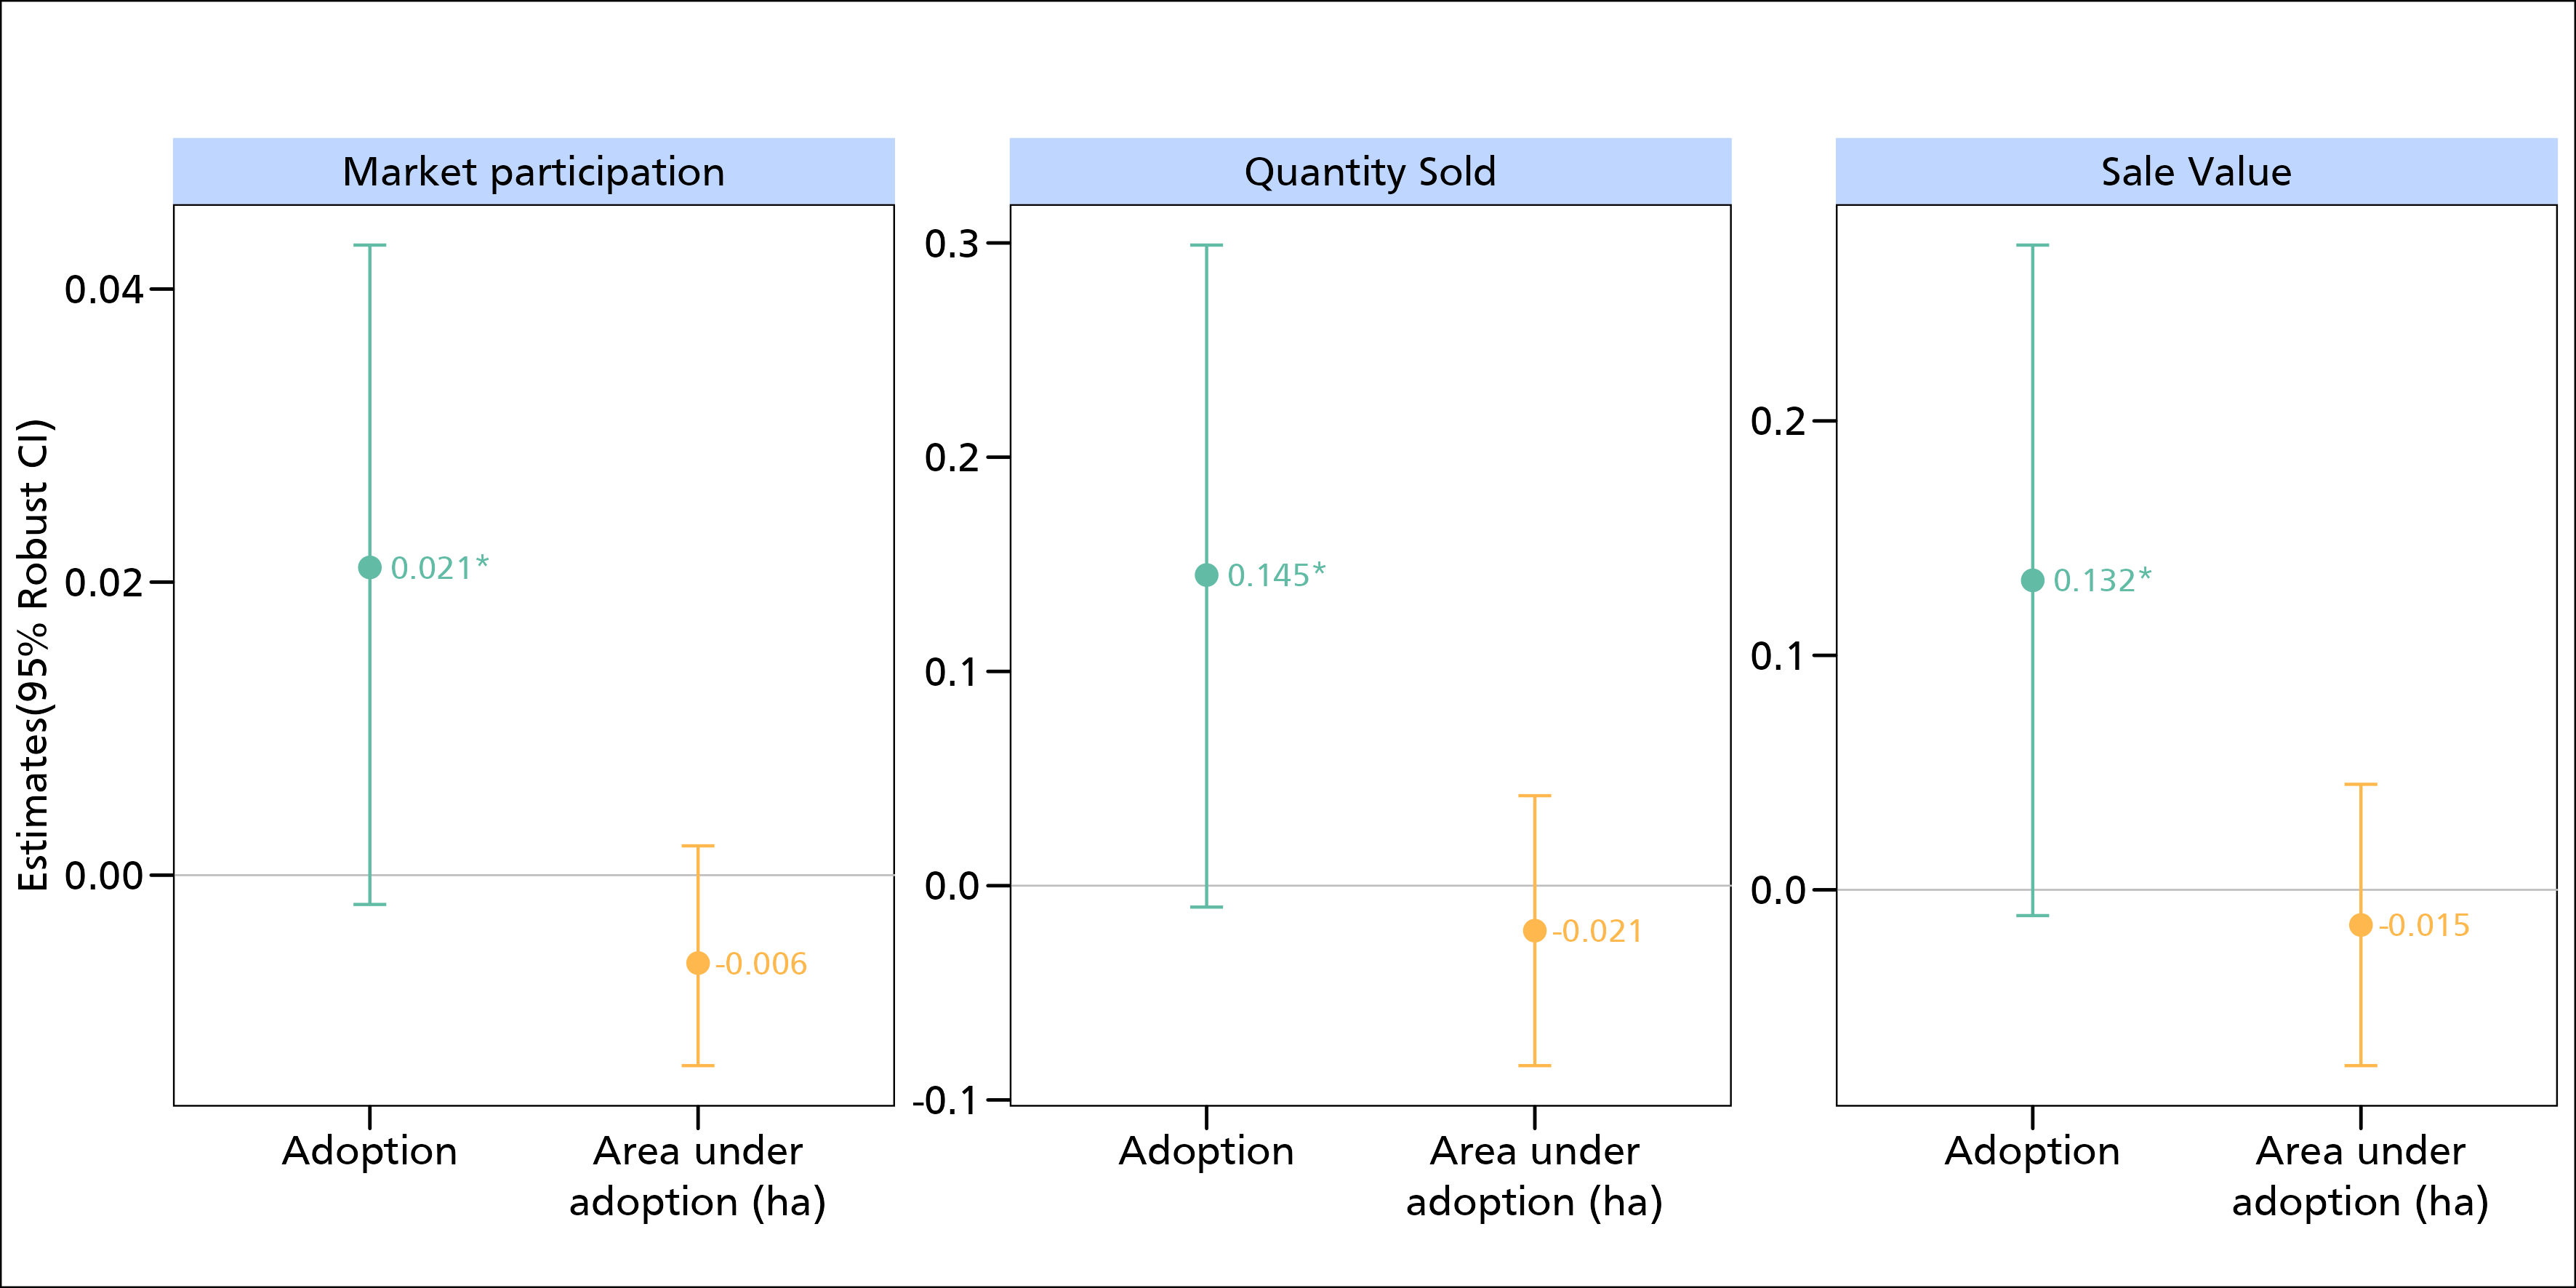
\includegraphics[width=\textwidth]{figures/fig_SM1.png}
\caption{OLS estimates of the relationship between adoption and commercialization}
\end{figure}

Note: Full models are reported in SM2. Robust standard errors in parentheses. Additional controls include age and educational level of the household head, dependency ratio, whether the household head is male, household size, cooperative membership, training, access to public and private extension, access to credits both in
\newpage
Estimating the relationship between adoption of improved groundnuts, production, production value and land productivity using the FE-OLS model (Figure S2), we obtain positive coefficients for all outcomes. When we consider adoption as a dummy, we observe production and productivity increases of about 540Kg and 285Kg/ha respectively. Considering the scale of adoption, we observe that adoption of improved climate-smart groundnut varieties increases groundnut production by 240Kg and land productivity by approximately 60Kg/ha. The magnitudes here are positive indicating that adoption both when considered as a dummy as well as extent increases yield, production, and production value. The smaller magnitudes here might be indicative of diminishing returns as early highlighted. The positive and significant estimates of the area under adoption variable aligns with the tenets of the non-separable agricultural household model where the production, consumption and ultimately commercialization decisions of households are non-separable. This suggests that households would only participate in markets to the extent that the household food production and consumption needs are met.

\begin{figure}[htbp]
\centering
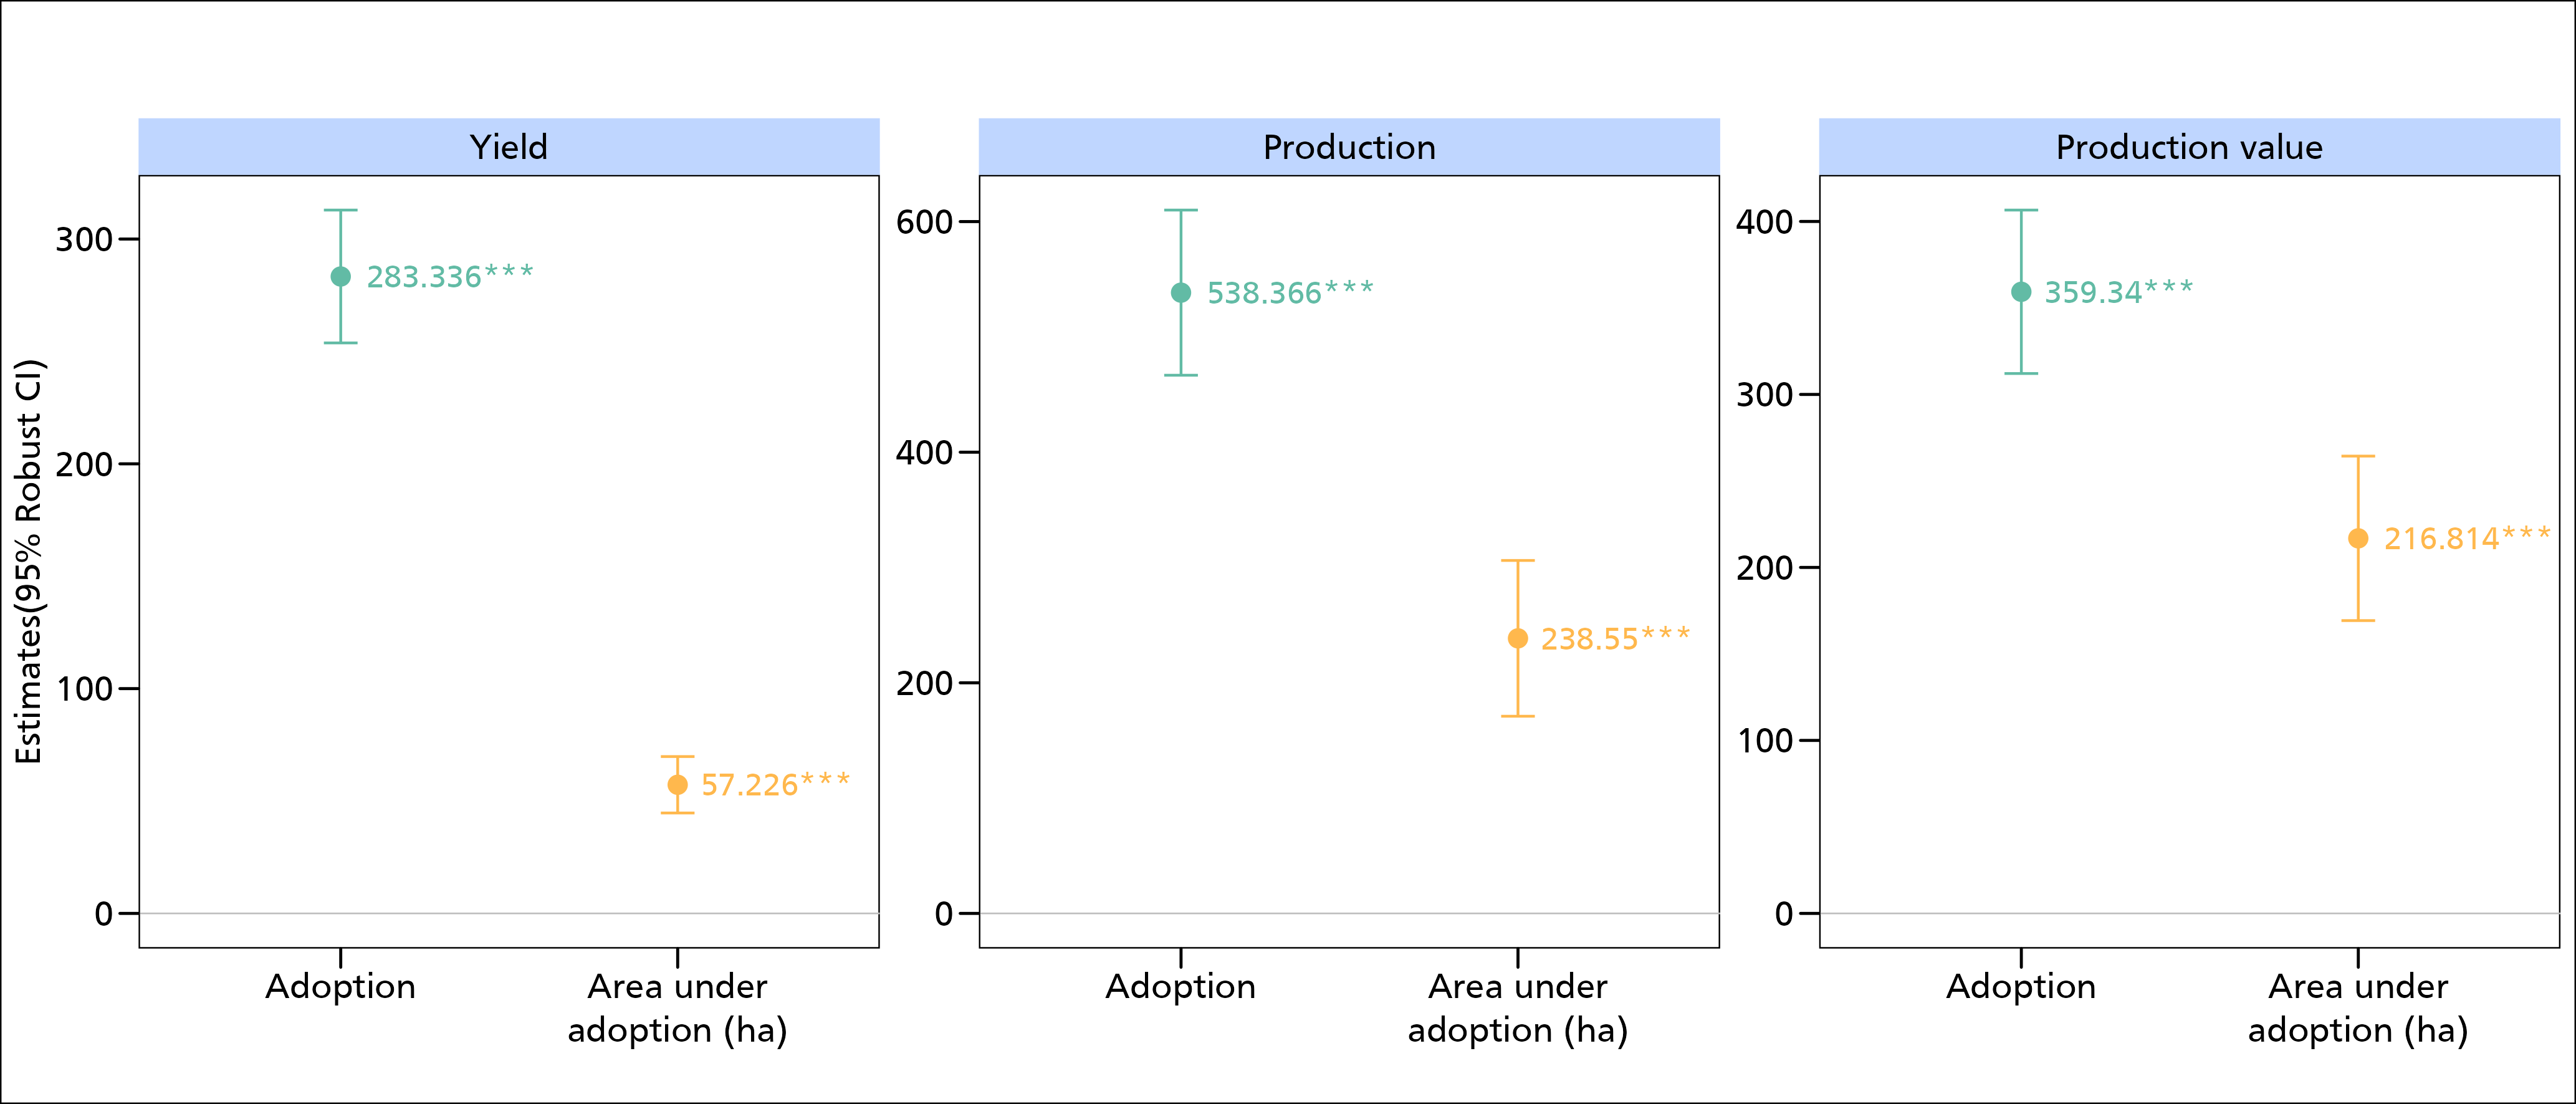
\includegraphics[width=\textwidth]{figures/fig_SM2.png}
\caption{OLS estimates of the relationship between adoption and commercialization}
\end{figure}

Note: Full models are reported in SM4. Robust standard errors in parentheses). Additional controls include age and educational level of the household head, dependency ratio, whether the household head is male, household size, cooperative membership, training, access to public and private extension, access to credits both in cash and kind, distance to nearest urban and village market, crop rotation, mixed cropping, labour, market price, input costs, area of cultivation, off-farm income and soil type (*** p\textless0.01, ** p\textless0.05, * p\textless0.1)

\newpage

\hypertarget{descriptive-statistics}{%
\section{Descriptive statistics}\label{descriptive-statistics}}

\begin{landscape}\begin{table}[!h]

\caption{\label{tab:unnamed-chunk-2}Descriptive statistics by year and adoption status}
\centering
\resizebox{\linewidth}{!}{
\fontsize{6}{8}\selectfont
\begin{tabular}[t]{lccccccccc}
\toprule
\multicolumn{1}{c}{ } & \multicolumn{3}{c}{\textbf{2017}, N = 2868} & \multicolumn{3}{c}{\textbf{2018}, N = 2868} & \multicolumn{3}{c}{\textbf{2019}, N = 2868} \\
\cmidrule(l{3pt}r{3pt}){2-4} \cmidrule(l{3pt}r{3pt}){5-7} \cmidrule(l{3pt}r{3pt}){8-10}
\textbf{Characteristic} & \textbf{Non-adopter}, N = 1,809 & \textbf{Adopter}, N = 1,059 & \textbf{p-value} & \textbf{Non-adopter}, N = 1,770 & \textbf{Adopter}, N = 1,098 & \textbf{p-value} & \textbf{Non-adopter}, N = 1,670 & \textbf{Adopter}, N = 1,198 & \textbf{p-value}\\
\midrule
Country &  &  & <0.001 &  &  & <0.001 &  &  & <0.001\\
\hspace{1em}Ghana & 327 (18\%) & 171 (16\%) &  & 353 (20\%) & 145 (13\%) &  & 340 (20\%) & 158 (13\%) & \\
\hspace{1em}Mali & 697 (39\%) & 143 (14\%) &  & 693 (39\%) & 147 (13\%) &  & 642 (38\%) & 198 (17\%) & \\
\hspace{1em}Nigeria & 785 (43\%) & 745 (70\%) &  & 724 (41\%) & 806 (73\%) &  & 688 (41\%) & 842 (70\%) & \\
Age of household head (years) & 48 (13) & 47 (11) & 0.073 & 49 (13) & 47 (11) & <0.001 & 50 (12) & 49 (12) & 0.14\\
\addlinespace
Sex of household head (dummy, male=1) & 1,681 (93\%) & 1,004 (95\%) & 0.047 & 1,629 (92\%) & 1,056 (96\%) & <0.001 & 1,546 (93\%) & 1,139 (95\%) & 0.007\\
Education level (Number of years) & 2.5 (3.8) & 3.4 (4.4) & <0.001 & 2.4 (3.8) & 3.6 (4.4) & <0.001 & 2.1 (3.3) & 3.9 (4.8) & <0.001\\
Household size (number of persons) & 12 (7) & 10 (6) & <0.001 & 12 (7) & 10 (6) & <0.001 & 13 (10) & 10 (7) & <0.001\\
Dependency ratio & 1.59 (1.10) & 1.77 (1.38) & 0.029 & 1.64 (1.15) & 1.69 (1.30) & 0.8 & 1.74 (1.32) & 1.95 (1.63) & 0.015\\
Farmers group membership (dummy) & 757 (42\%) & 551 (52\%) & <0.001 & 771 (44\%) & 537 (49\%) & 0.005 & 696 (42\%) & 518 (43\%) & 0.4\\
\addlinespace
Training on agriculture (dummy) & 591 (33\%) & 473 (45\%) & <0.001 & 557 (31\%) & 507 (46\%) & <0.001 & 530 (32\%) & 565 (47\%) & <0.001\\
Training on groundnut farming(dummy) & 1,020 (56\%) & 587 (55\%) & 0.6 & 1,001 (57\%) & 606 (55\%) & 0.5 & 629 (38\%) & 766 (64\%) & <0.001\\
Public agricultural extension service (number of visits) & 1.21 (1.66) & 3.32 (3.30) & <0.001 & 1.40 (1.84) & 2.94 (3.29) & <0.001 & 1.71 (1.90) & 2.47 (2.12) & <0.001\\
Private agricultural extension service (number of visits) & 0.58 (0.90) & 1.54 (1.89) & <0.001 & 0.62 (0.94) & 1.44 (1.88) & <0.001 & 1.11 (1.33) & 1.38 (1.57) & <0.001\\
Cash credit for groundnut farming (dummy) & 32 (1.8\%) & 24 (2.3\%) & 0.4 & 30 (1.7\%) & 26 (2.4\%) & 0.2 & 49 (2.9\%) & 76 (6.3\%) & <0.001\\
\addlinespace
Credit in kind for groundnut farming (dummy) & 62 (3.4\%) & 129 (12\%) & <0.001 & 54 (3.1\%) & 137 (12\%) & <0.001 & 87 (5.2\%) & 150 (13\%) & <0.001\\
Distance to the nearest urban market (km) & 15 (18) & 11 (11) & <0.001 & 15 (19) & 11 (11) & <0.001 & 13 (14) & 12 (14) & <0.001\\
Distance the nearest village market (km) & 3.8 (5.3) & 3.5 (3.7) & 0.004 & 3.9 (5.4) & 3.4 (3.6) & 0.003 & 4.8 (5.0) & 3.6 (4.5) & <0.001\\
Crop rotation (dummy) & 889 (49\%) & 397 (37\%) & <0.001 & 905 (51\%) & 381 (35\%) & <0.001 & 921 (55\%) & 393 (33\%) & <0.001\\
Mixed Crops (dummy) & 657 (36\%) & 448 (42\%) & 0.001 & 681 (38\%) & 424 (39\%) & >0.9 & 725 (43\%) & 542 (45\%) & 0.3\\
\addlinespace
Labor force (man.day) & 3.9 (5.1) & 6.5 (7.4) & <0.001 & 4.4 (5.5) & 5.6 (7.1) & <0.001 & 7 (9) & 7 (6) & <0.001\\
Unit selling price (USD/kg) & 0.53 (0.07) & 0.71 (0.08) & <0.001 & 0.53 (0.07) & 0.72 (0.08) & <0.001 & 0.53 (0.07) & 0.71 (0.09) & <0.001\\
Seed cost (USD/ha) & 8 (16) & 27 (19) & <0.001 & 8 (17) & 25 (20) & <0.001 & 20 (21) & 23 (19) & <0.001\\
Fertilizer cost (USD/ha) & 17 (29) & 53 (39) & <0.001 & 18 (30) & 49 (40) & <0.001 & 19 (28) & 49 (39) & <0.001\\
Pesticide cost (USD/ha) & 4 (8) & 14 (14) & <0.001 & 4 (8) & 13 (14) & <0.001 & 6 (13) & 11 (11) & <0.001\\
\addlinespace
Labor cost (USD/ha) & 21 (33) & 49 (41) & <0.001 & 24 (34) & 43 (41) & <0.001 & 50 (49) & 50 (41) & 0.031\\
Groundnut area (ha) & 1.44 (1.47) & 1.81 (1.62) & <0.001 & 1.49 (1.46) & 1.72 (1.64) & <0.001 & 1.60 (1.47) & 1.72 (1.32) & <0.001\\
Off-farm income (dummy) & 80 (4.4\%) & 190 (18\%) & <0.001 & 85 (4.8\%) & 185 (17\%) & <0.001 & 142 (8.5\%) & 199 (17\%) & <0.001\\
Clay soil (dummy) & 279 (15\%) & 164 (15\%) & >0.9 & 271 (15\%) & 172 (16\%) & 0.8 & 282 (17\%) & 207 (17\%) & 0.8\\
Sandy-clay soil (dummy) & 987 (55\%) & 595 (56\%) & 0.4 & 977 (55\%) & 605 (55\%) & >0.9 & 740 (44\%) & 516 (43\%) & 0.5\\
\addlinespace
Silty soil (dummy) & 281 (16\%) & 162 (15\%) & 0.9 & 278 (16\%) & 165 (15\%) & 0.6 & 306 (18\%) & 200 (17\%) & 0.3\\
\bottomrule
\multicolumn{10}{l}{\rule{0pt}{1em}\textsuperscript{1} n (\%); Mean (SD)}\\
\multicolumn{10}{l}{\rule{0pt}{1em}\textsuperscript{2} Pearson's Chi-squared test; Wilcoxon rank sum test}\\
\end{tabular}}
\end{table}
\end{landscape}
\newpage

\hypertarget{pooled-ols-regressions}{%
\section{Pooled OLS Regressions}\label{pooled-ols-regressions}}

\begingroup\fontsize{7}{9}\selectfont

\begin{longtable}[t]{lrrr}
\caption{\label{tab:unnamed-chunk-3}Full OLS estimates of the relationship between adoption and commercialization(Adoption)}\\
\toprule
variables & Sellers & Quantity Sold & Sales value\\
\midrule
\endfirsthead
\caption[]{\label{tab:unnamed-chunk-3}Full OLS estimates of the relationship between adoption and commercialization(Adoption) \textit{(continued)}}\\
\toprule
variables & Sellers & Quantity Sold & Sales value\\
\midrule
\endhead

\endfoot
\bottomrule
\endlastfoot
Adoption dummy & 0.021* & 0.145* & 0.132*\\
 & 0.012 & 0.079 & 0.073\\
Age of household head (years) & -0.001** & -0.006** & -0.005***\\
 & 0.000 & 0.002 & 0.002\\
Sex of household head (dummy, male=1) & -0.012 & 0.105 & 0.112\\
 & 0.020 & 0.129 & 0.118\\
Education level (Number of years) & 0.001 & -0.005 & -0.005\\
 & 0.001 & 0.006 & 0.005\\
Household size (number of persons) & 0.000 & 0.015*** & 0.015***\\
 & 0.001 & 0.005 & 0.004\\
Farmers group membership (dummy) & 0.022*** & 0.132*** & 0.120***\\
 & 0.004 & 0.029 & 0.027\\
Training on agriculture (dummy) & -0.057*** & -0.320*** & -0.282***\\
 & 0.011 & 0.074 & 0.068\\
Training on groundnut farming (dummy) & -0.021*** & -0.154*** & -0.143***\\
 & 0.004 & 0.025 & 0.023\\
Public agricultural extension service (number of visits) & 0.001 & -0.017 & -0.018\\
 & 0.002 & 0.014 & 0.013\\
Private agricultural extension service (number of visits) & 0.007** & 0.034* & 0.027\\
 & 0.003 & 0.020 & 0.019\\
Cash credit for groundnut farming (dummy) & 0.011 & 0.034 & 0.026\\
 & 0.020 & 0.140 & 0.130\\
Credit in kind for groundnut farming (dummy) & -0.008 & 0.039 & 0.043\\
 & 0.012 & 0.088 & 0.082\\
Distance to the nearest urban market (km) & -0.002*** & -0.015*** & -0.014***\\
 & 0.000 & 0.002 & 0.002\\
Distance the nearest village market (km) & -0.004*** & -0.021*** & -0.019***\\
 & 0.001 & 0.007 & 0.007\\
Crop rotation (dummy) & 0.010 & 0.085 & 0.078\\
 & 0.010 & 0.063 & 0.057\\
Mixed Crops (dummy) & 0.003 & -0.095* & -0.097**\\
 & 0.008 & 0.051 & 0.047\\
Labor force (man.day) & 0.002*** & 0.024*** & 0.023***\\
 & 0.001 & 0.004 & 0.004\\
Unit selling price (USD/kg) & 0.068 & 0.579** & 2.001***\\
 & 0.042 & 0.286 & 0.264\\
Seed cost (USD/ha) & 0.001*** & 0.010*** & 0.009***\\
 & 0.000 & 0.002 & 0.002\\
Fertilizer cost (USD/ha) & 0.000 & 0.001* & 0.001*\\
 & 0.000 & 0.001 & 0.001\\
Pesticide cost (USD/ha) & -0.000 & 0.003 & 0.003\\
 & 0.000 & 0.002 & 0.002\\
Labor cost (USD/ha) & 0.000*** & 0.002*** & 0.002***\\
 & 0.000 & 0.001 & 0.001\\
Groundnut area (ha) & 0.019*** & 0.347*** & 0.335***\\
 & 0.003 & 0.022 & 0.021\\
Off-farm income (dummy) & -0.033*** & -0.151** & -0.135**\\
 & 0.010 & 0.074 & 0.069\\
Dependency ratio & 0.001 & -0.002 & -0.003\\
 & 0.003 & 0.019 & 0.017\\
Clay soil (dummy) & -0.008 & -0.097 & -0.095\\
 & 0.011 & 0.077 & 0.071\\
Sandy-clay soil (dummy) & 0.007 & 0.035 & 0.031\\
 & 0.009 & 0.061 & 0.056\\
Silty soil (dummy) & 0.008 & 0.052 & 0.046\\
 & 0.011 & 0.076 & 0.070\\
Observations & 8,604 & 8,604 & 8,604\\
R-squared & 0.274 & 0.421 & 0.451\\
F test & 13.95 & 30.48 & 37.56\\*
\end{longtable}
\endgroup{}
\newpage

\begingroup\fontsize{7}{9}\selectfont

\begin{longtable}[t]{lrrr}
\caption{\label{tab:unnamed-chunk-4}Full OLS estimates of the relationship between adoption and commercialization (Area under Adoption)}\\
\toprule
variables & Production & Production value & Yield\\
\midrule
\endfirsthead
\caption[]{\label{tab:unnamed-chunk-4}Full OLS estimates of the relationship between adoption and commercialization (Area under Adoption) \textit{(continued)}}\\
\toprule
variables & Production & Production value & Yield\\
\midrule
\endhead

\endfoot
\bottomrule
\endlastfoot
Area under adoption (ha) & -0.006 & -0.021 & -0.015\\
 & 0.004 & 0.032 & 0.031\\
Age of household head (years) & -0.001** & -0.006** & -0.005***\\
 & 0.000 & 0.002 & 0.002\\
Sex of household head (dummy, male=1) & -0.011 & 0.110 & 0.116\\
 & 0.020 & 0.129 & 0.118\\
Education level (Number of years) & 0.001 & -0.005 & -0.006\\
 & 0.001 & 0.006 & 0.005\\
Household size (number of persons) & 0.000 & 0.014*** & 0.014***\\
 & 0.001 & 0.005 & 0.004\\
Farmers group membership (dummy) & 0.022*** & 0.132*** & 0.120***\\
 & 0.004 & 0.029 & 0.027\\
Training on agriculture (dummy) & -0.056*** & -0.319*** & -0.282***\\
 & 0.011 & 0.074 & 0.068\\
Training on groundnut farming (dummy) & -0.021*** & -0.155*** & -0.144***\\
 & 0.004 & 0.025 & 0.023\\
Public agricultural extension service (number of visits) & 0.001 & -0.015 & -0.016\\
 & 0.002 & 0.014 & 0.013\\
Private agricultural extension service (number of visits) & 0.008*** & 0.042** & 0.033*\\
 & 0.003 & 0.020 & 0.019\\
Cash credit for groundnut farming (dummy) & 0.011 & 0.038 & 0.030\\
 & 0.020 & 0.140 & 0.131\\
Credit in kind for groundnut farming (dummy) & -0.006 & 0.052 & 0.053\\
 & 0.012 & 0.087 & 0.082\\
Distance to the nearest urban market (km) & -0.002*** & -0.015*** & -0.014***\\
 & 0.000 & 0.002 & 0.002\\
Distance the nearest village market (km) & -0.004*** & -0.021*** & -0.019***\\
 & 0.001 & 0.007 & 0.007\\
Crop rotation (dummy) & 0.009 & 0.080 & 0.074\\
 & 0.010 & 0.063 & 0.058\\
Mixed Crops (dummy) & 0.002 & -0.100* & -0.102**\\
 & 0.008 & 0.051 & 0.047\\
Labor force (man.day) & 0.002*** & 0.023*** & 0.022***\\
 & 0.001 & 0.004 & 0.004\\
Unit selling price (USD/kg) & 0.134*** & 0.982*** & 2.357***\\
 & 0.034 & 0.235 & 0.218\\
Seed cost (USD/ha) & 0.001*** & 0.010*** & 0.009***\\
 & 0.000 & 0.002 & 0.002\\
Fertilizer cost (USD/ha) & 0.000 & 0.002** & 0.002**\\
 & 0.000 & 0.001 & 0.001\\
Pesticide cost (USD/ha) & -0.000 & 0.004 & 0.004*\\
 & 0.000 & 0.002 & 0.002\\
Labor cost (USD/ha) & 0.000*** & 0.002*** & 0.002***\\
 & 0.000 & 0.001 & 0.001\\
Groundnut area (ha) & 0.022*** & 0.355*** & 0.342***\\
 & 0.003 & 0.022 & 0.021\\
Off-farm income (dummy) & -0.033*** & -0.150** & -0.134*\\
 & 0.010 & 0.074 & 0.069\\
Dependency ratio & 0.001 & -0.003 & -0.003\\
 & 0.003 & 0.019 & 0.017\\
Clay soil (dummy) & -0.009 & -0.101 & -0.099\\
 & 0.011 & 0.077 & 0.071\\
Sandy-clay soil (dummy) & 0.006 & 0.032 & 0.028\\
 & 0.009 & 0.060 & 0.055\\
Silty soil (dummy) & 0.008 & 0.053 & 0.046\\
 & 0.011 & 0.076 & 0.070\\
Observations & 8,604 & 8,604 & 8,604\\
R-squared & 0.273 & 0.421 & 0.451\\
F test & 14.32 & 31.28 & 38.78\\*
\end{longtable}
\endgroup{}

\newpage

\begingroup\fontsize{7}{9}\selectfont

\begin{longtable}[t]{lrrr}
\caption{\label{tab:unnamed-chunk-5} Full OLS estimates of the relationship between adoption, production and yields(Adoption)}\\
\toprule
variables & Production & Production value & Yield\\
\midrule
\endfirsthead
\caption[]{\label{tab:unnamed-chunk-5} Full OLS estimates of the relationship between adoption, production and yields(Adoption) \textit{(continued)}}\\
\toprule
variables & Production & Production value & Yield\\
\midrule
\endhead

\endfoot
\bottomrule
\endlastfoot
Adoption dummy & 538.366*** & 359.340*** & 283.336***\\
 & 36.536 & 24.099 & 15.075\\
Age of household head (years) & 0.226 & 0.246 & -0.023\\
 & 0.882 & 0.625 & 0.374\\
Sex of household head (dummy, male=1) & -17.450 & -20.938 & -24.355\\
 & 31.798 & 23.338 & 17.706\\
Education level (Number of years) & 0.573 & -0.462 & 1.681\\
 & 2.929 & 2.113 & 1.329\\
Household size (number of persons) & -2.087 & -3.346** & 0.531\\
 & 1.918 & 1.312 & 0.633\\
Farmers group membership (dummy) & 27.503* & 23.696** & 1.717\\
 & 14.436 & 10.143 & 5.305\\
Training on agriculture (dummy) & 20.058 & 10.166 & 12.945\\
 & 28.123 & 19.713 & 11.464\\
Training on groundnut farming (dummy) & -2.803 & -3.008 & -2.129\\
 & 9.558 & 6.533 & 4.027\\
Public agricultural extension service (number of visits) & -10.965 & -9.267* & -7.113**\\
 & 7.583 & 5.383 & 2.889\\
Private agricultural extension service (number of visits) & -20.005** & -13.667** & -3.053\\
 & 9.408 & 6.454 & 3.826\\
Cash credit for groundnut farming (dummy) & -116.583* & -96.283** & -3.990\\
 & 62.411 & 42.370 & 27.589\\
Credit in kind for groundnut farming (dummy) & 19.798 & 39.725 & -8.167\\
 & 52.308 & 37.817 & 19.779\\
Distance to the nearest urban market (km) & -0.254 & -0.150 & 0.039\\
 & 0.828 & 0.553 & 0.353\\
Distance the nearest village market (km) & -3.361* & -2.097* & -1.617**\\
 & 1.840 & 1.198 & 0.795\\
Crop rotation (dummy) & -54.106* & -50.565** & 1.007\\
 & 27.676 & 19.779 & 11.600\\
Mixed Crops (dummy) & 40.551* & 32.475** & -1.605\\
 & 21.514 & 15.265 & 9.425\\
Labor force (man.day) & -4.390 & -3.713** & -1.619**\\
 & 2.721 & 1.808 & 0.788\\
Unit selling price (USD/kg) & 36.726 & 1,208.590*** & 93.809*\\
 & 128.183 & 90.647 & 55.544\\
Seed cost (USD/ha) & -0.542 & -0.338 & -0.371\\
 & 0.569 & 0.402 & 0.257\\
Fertilizer cost (USD/ha) & -1.346*** & -1.273*** & -0.004\\
 & 0.440 & 0.322 & 0.199\\
Pesticide cost (USD/ha) & 2.260* & 2.177** & 0.024\\
 & 1.289 & 0.999 & 0.531\\
Labor cost (USD/ha) & 0.075 & 0.043 & -0.082\\
 & 0.265 & 0.191 & 0.131\\
Groundnut area (ha) & 698.176*** & 436.072*** & 1.376\\
 & 20.072 & 13.993 & 3.300\\
Off-farm income (dummy) & -15.131 & -9.056 & -21.645\\
 & 39.174 & 29.191 & 18.076\\
Dependency ratio & -10.922 & -9.494* & -1.563\\
 & 7.625 & 5.439 & 3.538\\
Clay soil (dummy) & 6.092 & 0.292 & 3.708\\
 & 29.406 & 20.300 & 13.795\\
Sandy-clay soil (dummy) & 28.195 & 20.606 & -1.381\\
 & 25.243 & 17.693 & 11.221\\
Silty soil (dummy) & 20.218 & 14.880 & 12.882\\
 & 30.870 & 21.598 & 13.986\\
Observations & 8,604 & 8,604 & 8,604\\
R-squared & 0.616 & 0.594 & 0.181\\
F test & 69.22 & 73.12 & 26.48\\*
\end{longtable}
\endgroup{}

\newpage

\begingroup\fontsize{7}{9}\selectfont

\begin{longtable}[t]{lrrr}
\caption{\label{tab:unnamed-chunk-6}OLS estimates of the relationship between adoption, production and yields(Area under Adoption)}\\
\toprule
variables & Production & Production value & Yield\\
\midrule
\endfirsthead
\caption[]{\label{tab:unnamed-chunk-6}OLS estimates of the relationship between adoption, production and yields(Area under Adoption) \textit{(continued)}}\\
\toprule
variables & Production & Production value & Yield\\
\midrule
\endhead

\endfoot
\bottomrule
\endlastfoot
Area under adoption (ha) & 238.550*** & 216.814*** & 57.226***\\
 & 34.459 & 24.253 & 6.403\\
Age of household head (years) & 0.377 & 0.374 & 0.025\\
 & 0.875 & 0.611 & 0.380\\
Sex of household head (dummy, male=1) & -17.307 & -23.796 & -20.776\\
 & 29.621 & 20.843 & 17.751\\
Education level (Number of years) & 2.728 & 1.428 & 2.280*\\
 & 2.916 & 2.076 & 1.354\\
Household size (number of persons) & 0.104 & -1.326 & 1.023\\
 & 1.852 & 1.243 & 0.641\\
Farmers group membership (dummy) & 23.024 & 19.604* & 0.668\\
 & 14.530 & 10.143 & 5.411\\
Training on agriculture (dummy) & 19.017 & 8.794 & 13.199\\
 & 28.199 & 19.422 & 11.653\\
Training on groundnut farming (dummy) & -6.485 & -5.155 & -4.435\\
 & 9.625 & 6.519 & 4.090\\
Public agricultural extension service (number of visits) & -5.811 & -6.431 & -3.685\\
 & 7.401 & 5.123 & 2.924\\
Private agricultural extension service (number of visits) & -10.123 & -10.434* & 6.138\\
 & 9.116 & 6.215 & 3.799\\
Cash credit for groundnut farming (dummy) & -87.350 & -74.251* & 8.406\\
 & 63.173 & 42.902 & 28.328\\
Credit in kind for groundnut farming (dummy) & -8.897 & 6.830 & -6.967\\
 & 50.662 & 35.263 & 20.115\\
Distance to the nearest urban market (km) & -0.735 & -0.486 & -0.196\\
 & 0.826 & 0.541 & 0.363\\
Distance the nearest village market (km) & -3.326* & -2.099* & -1.568**\\
 & 1.806 & 1.139 & 0.794\\
Crop rotation (dummy) & -42.921 & -38.056** & 0.911\\
 & 26.863 & 18.900 & 11.740\\
Mixed Crops (dummy) & 34.291 & 30.585** & -7.613\\
 & 21.331 & 14.868 & 9.562\\
Labor force (man.day) & -4.084 & -3.021 & -2.037**\\
 & 2.927 & 1.994 & 0.808\\
Unit selling price (USD/kg) & 512.083*** & 1,339.478*** & 565.109***\\
 & 133.797 & 96.971 & 49.594\\
Seed cost (USD/ha) & 0.128 & 0.059 & 0.042\\
 & 0.546 & 0.370 & 0.259\\
Fertilizer cost (USD/ha) & -0.846** & -0.963*** & 0.288\\
 & 0.431 & 0.312 & 0.201\\
Pesticide cost (USD/ha) & 2.188* & 1.732* & 0.456\\
 & 1.325 & 1.024 & 0.540\\
Labor cost (USD/ha) & 0.010 & -0.006 & -0.110\\
 & 0.257 & 0.179 & 0.133\\
Groundnut area (ha) & 634.558*** & 376.027*** & -11.249***\\
 & 20.141 & 13.418 & 3.596\\
Off-farm income (dummy) & -3.625 & 0.179 & -17.434\\
 & 38.674 & 28.513 & 18.365\\
Dependency ratio & -7.874 & -6.761 & -0.786\\
 & 7.614 & 5.353 & 3.592\\
Clay soil (dummy) & 28.503 & 22.644 & 6.733\\
 & 29.032 & 19.653 & 14.049\\
Sandy-clay soil (dummy) & 45.222* & 36.851** & 1.791\\
 & 24.917 & 17.077 & 11.460\\
Silty soil (dummy) & 26.747 & 20.009 & 15.403\\
 & 30.838 & 21.038 & 14.258\\
Observations & 8,604 & 8,604 & 8,604\\
R-squared & 0.622 & 0.613 & 0.156\\
F test & 64.51 & 71.32 & 16.55\\*
\end{longtable}
\endgroup{}
\newpage

\hypertarget{panel-regression}{%
\section{Panel Regression}\label{panel-regression}}

\begingroup\fontsize{7}{9}\selectfont

\begin{longtable}[t]{lrrr}
\caption{\label{tab:unnamed-chunk-7}Full 2SLS estimates of the relationship between adoption and commercialization(Adoption)}\\
\toprule
variables & Production & Production value & Yield\\
\midrule
\endfirsthead
\caption[]{\label{tab:unnamed-chunk-7}Full 2SLS estimates of the relationship between adoption and commercialization(Adoption) \textit{(continued)}}\\
\toprule
variables & Production & Production value & Yield\\
\midrule
\endhead

\endfoot
\bottomrule
\endlastfoot
Area under adoption (ha) & 238.550*** & 216.814*** & 57.226***\\
 & 34.459 & 24.253 & 6.403\\
Age of household head (years) & 0.377 & 0.374 & 0.025\\
 & 0.875 & 0.611 & 0.380\\
Sex of household head (dummy, male=1) & -17.307 & -23.796 & -20.776\\
 & 29.621 & 20.843 & 17.751\\
Education level (Number of years) & 2.728 & 1.428 & 2.280*\\
 & 2.916 & 2.076 & 1.354\\
Household size (number of persons) & 0.104 & -1.326 & 1.023\\
 & 1.852 & 1.243 & 0.641\\
Farmers group membership (dummy) & 23.024 & 19.604* & 0.668\\
 & 14.530 & 10.143 & 5.411\\
Training on agriculture (dummy) & 19.017 & 8.794 & 13.199\\
 & 28.199 & 19.422 & 11.653\\
Training on groundnut farming (dummy) & -6.485 & -5.155 & -4.435\\
 & 9.625 & 6.519 & 4.090\\
Public agricultural extension service (number of visits) & -5.811 & -6.431 & -3.685\\
 & 7.401 & 5.123 & 2.924\\
Private agricultural extension service (number of visits) & -10.123 & -10.434* & 6.138\\
 & 9.116 & 6.215 & 3.799\\
Cash credit for groundnut farming (dummy) & -87.350 & -74.251* & 8.406\\
 & 63.173 & 42.902 & 28.328\\
Credit in kind for groundnut farming (dummy) & -8.897 & 6.830 & -6.967\\
 & 50.662 & 35.263 & 20.115\\
Distance to the nearest urban market (km) & -0.735 & -0.486 & -0.196\\
 & 0.826 & 0.541 & 0.363\\
Distance the nearest village market (km) & -3.326* & -2.099* & -1.568**\\
 & 1.806 & 1.139 & 0.794\\
Crop rotation (dummy) & -42.921 & -38.056** & 0.911\\
 & 26.863 & 18.900 & 11.740\\
Mixed Crops (dummy) & 34.291 & 30.585** & -7.613\\
 & 21.331 & 14.868 & 9.562\\
Labor force (man.day) & -4.084 & -3.021 & -2.037**\\
 & 2.927 & 1.994 & 0.808\\
Unit selling price (USD/kg) & 512.083*** & 1,339.478*** & 565.109***\\
 & 133.797 & 96.971 & 49.594\\
Seed cost (USD/ha) & 0.128 & 0.059 & 0.042\\
 & 0.546 & 0.370 & 0.259\\
Fertilizer cost (USD/ha) & -0.846** & -0.963*** & 0.288\\
 & 0.431 & 0.312 & 0.201\\
Pesticide cost (USD/ha) & 2.188* & 1.732* & 0.456\\
 & 1.325 & 1.024 & 0.540\\
Labor cost (USD/ha) & 0.010 & -0.006 & -0.110\\
 & 0.257 & 0.179 & 0.133\\
Groundnut area (ha) & 634.558*** & 376.027*** & -11.249***\\
 & 20.141 & 13.418 & 3.596\\
Off-farm income (dummy) & -3.625 & 0.179 & -17.434\\
 & 38.674 & 28.513 & 18.365\\
Dependency ratio & -7.874 & -6.761 & -0.786\\
 & 7.614 & 5.353 & 3.592\\
Clay soil (dummy) & 28.503 & 22.644 & 6.733\\
 & 29.032 & 19.653 & 14.049\\
Sandy-clay soil (dummy) & 45.222* & 36.851** & 1.791\\
 & 24.917 & 17.077 & 11.460\\
Silty soil (dummy) & 26.747 & 20.009 & 15.403\\
 & 30.838 & 21.038 & 14.258\\
Observations & 8,604 & 8,604 & 8,604\\
R-squared & 0.622 & 0.613 & 0.156\\
F test & 64.51 & 71.32 & 16.55\\*
\end{longtable}
\endgroup{}
\newpage

\begingroup\fontsize{7}{9}\selectfont

\begin{longtable}[t]{lrrrlrr}
\caption{\label{tab:unnamed-chunk-8}Full 2SLS estimates of the relationship between adoption and commercialization}\\
\toprule
variables & FE-MP & RE-MP & FE-QS & RE-QS & FE-SV & RE-SV\\
\midrule
\endfirsthead
\caption[]{\label{tab:unnamed-chunk-8}Full 2SLS estimates of the relationship between adoption and commercialization \textit{(continued)}}\\
\toprule
variables & FE-MP & RE-MP & FE-QS & RE-QS & FE-SV & RE-SV\\
\midrule
\endhead

\endfoot
\bottomrule
\endlastfoot
Adoption dummy & 0.064*** & 0.053*** & 0.594*** & 0.544*** & 0.570*** & 0.526***\\
 & (0.020) & (0.018) & (0.134) & (0.120) & (0.124) & (0.110)\\
Age of household head (years) & 0.002 & -0.001* & -0.011 & -0.006** & -0.013 & -0.005**\\
 & (0.003) & (0.000) & (0.024) & (0.003) & (0.022) & (0.003)\\
Sex of household head (dummy, male=1) &  & -0.011 &  & 0.115 &  & 0.121\\
 &  & (0.020) &  & (0.137) &  & (0.126)\\
Education level (Number of years) &  & 0.001 &  & -0.005 &  & -0.006\\
 &  & (0.001) &  & (0.009) &  & (0.008)\\
Household size (number of persons) & 0.002*** & 0.001* & 0.027*** & 0.020*** & 0.026*** & 0.019***\\
 & (0.001) & (0.001) & (0.005) & (0.004) & (0.004) & (0.004)\\
Farmers group membership (dummy) & 0.022*** & 0.023*** & 0.124*** & 0.132*** & 0.111*** & 0.119***\\
 & (0.005) & (0.004) & (0.035) & (0.028) & (0.032) & (0.026)\\
Training on agriculture (dummy) & -0.043*** & -0.052*** & -0.314*** & -0.318*** & -0.287*** & -0.285***\\
 & (0.011) & (0.009) & (0.078) & (0.065) & (0.072) & (0.059)\\
Training on groundnut farming (dummy) & -0.025*** & -0.023*** & -0.176*** & -0.166*** & -0.162*** & -0.153***\\
 & (0.003) & (0.003) & (0.023) & (0.021) & (0.021) & (0.019)\\
Public agricultural extension service (number of visits) & 0.002 & 0.002 & -0.024 & -0.020 & -0.025 & -0.021\\
 & (0.002) & (0.002) & (0.016) & (0.014) & (0.015) & (0.013)\\
Private agricultural extension service (number of visits) & 0.003 & 0.004 & 0.045* & 0.026 & 0.042* & 0.021\\
 & (0.003) & (0.003) & (0.024) & (0.020) & (0.022) & (0.019)\\
Cash credit for groundnut farming (dummy) & -0.010 & 0.000 & -0.186 & -0.076 & -0.193 & -0.083\\
 & (0.023) & (0.020) & (0.156) & (0.136) & (0.144) & (0.125)\\
Credit in kind for groundnut farming (dummy) & -0.044*** & -0.026* & -0.046 & -0.019 & -0.022 & -0.006\\
 & (0.016) & (0.014) & (0.109) & (0.094) & (0.100) & (0.086)\\
Distance to the nearest urban market (km) & -0.000 & -0.001*** & -0.003 & -0.009*** & -0.003 & -0.008***\\
 & (0.000) & (0.000) & (0.002) & (0.002) & (0.002) & (0.002)\\
Distance the nearest village market (km) & -0.003*** & -0.003*** & -0.013** & -0.017*** & -0.011* & -0.015***\\
 & (0.001) & (0.001) & (0.006) & (0.005) & (0.006) & (0.005)\\
Crop rotation (dummy) & -0.023** & -0.005 & -0.144** & -0.016 & -0.135** & -0.014\\
 & (0.011) & (0.009) & (0.072) & (0.061) & (0.066) & (0.056)\\
Mixed Crops (dummy) & 0.004 & 0.003 & -0.063 & -0.079 & -0.066 & -0.080*\\
 & (0.009) & (0.007) & (0.061) & (0.050) & (0.056) & (0.046)\\
Labor force (man.day) & 0.002*** & 0.002*** & 0.027*** & 0.026*** & 0.026*** & 0.025***\\
 & (0.001) & (0.001) & (0.005) & (0.004) & (0.004) & (0.004)\\
Unit selling price (USD/kg) & 0.009 & 0.012 & -0.134 & -0.180 & 1.301*** & 1.249***\\
 & (0.054) & (0.050) & (0.365) & (0.338) & (0.336) & (0.311)\\
Seed cost (USD/ha) & 0.002*** & 0.002*** & 0.011*** & 0.010*** & 0.010*** & 0.009***\\
 & (0.000) & (0.000) & (0.002) & (0.001) & (0.001) & (0.001)\\
Fertilizer cost (USD/ha) & 0.000 & 0.000 & 0.001 & 0.001 & 0.001 & 0.001\\
 & (0.000) & (0.000) & (0.001) & (0.001) & (0.001) & (0.001)\\
Pesticide cost (USD/ha) & -0.001*** & -0.001** & -0.005 & -0.002 & -0.004 & -0.001\\
 & (0.000) & (0.000) & (0.003) & (0.003) & (0.003) & (0.002)\\
Labor cost (USD/ha) & 0.000*** & 0.000*** & 0.002*** & 0.002*** & 0.002*** & 0.002***\\
 & (0.000) & (0.000) & (0.001) & (0.001) & (0.001) & (0.001)\\
Groundnut area (ha) & 0.003 & 0.013*** & 0.198*** & 0.282*** & 0.195*** & 0.274***\\
 & (0.003) & (0.003) & (0.023) & (0.019) & (0.021) & (0.017)\\
Off-farm income (dummy) & -0.020 & -0.027** & -0.035 & -0.101 & -0.024 & -0.088\\
 & (0.014) & (0.012) & (0.098) & (0.083) & (0.090) & (0.076)\\
Dependency ratio & 0.002 & 0.001 & 0.013 & 0.003 & 0.012 & 0.003\\
 & (0.003) & (0.003) & (0.022) & (0.018) & (0.020) & (0.016)\\
Clay soil (dummy) & -0.016 & -0.012 & -0.161* & -0.120 & -0.155* & -0.116*\\
 & (0.013) & (0.011) & (0.087) & (0.073) & (0.080) & (0.068)\\
Sandy-clay soil (dummy) & 0.006 & 0.006 & 0.052 & 0.036 & 0.048 & 0.032\\
 & (0.010) & (0.009) & (0.068) & (0.059) & (0.063) & (0.054)\\
Silty soil (dummy) & -0.004 & 0.002 & -0.032 & 0.010 & -0.033 & 0.007\\
 & (0.013) & (0.011) & (0.087) & (0.073) & (0.080) & (0.067)\\
Constant & 0.841*** & 0.987*** & 6.998*** & 7.194*** & 5.742*** & 5.831***\\
 & (0.183) & (0.053) & (1.244) & (0.361) & (1.144) & (0.331)\\
Observations & 8,604 & 8,604 & 8,604 & 8,604 & 8,604 & 8,604\\
Number of id & 2,868 & 2,868 & 2,868 & 2,868 & 2,868 & 2,868\\
District FE & YES & YES & YES & YES & YES & YES\\
Year FE & YES & YES & YES & YES & YES & YES\\
Standard errors in parentheses &  &  &  &  &  & \\
*** p<0.01, ** p<0.05, * p<0.1 &  &  &  &  &  & \\*
\end{longtable}
\endgroup{}

\newpage

\begin{landscape}\begingroup\fontsize{7}{9}\selectfont

\begin{longtable}[t]{lrrrlrr}
\caption{\label{tab:unnamed-chunk-9}Full 2SLS estimates of the relationship between adoption (Area), production and yields}\\
\toprule
variables & FE-MP & RE-MP & FE-QS & RE-QS & FE-SV & RE-SV\\
\midrule
\endfirsthead
\caption[]{\label{tab:unnamed-chunk-9}Full 2SLS estimates of the relationship between adoption (Area), production and yields \textit{(continued)}}\\
\toprule
variables & FE-MP & RE-MP & FE-QS & RE-QS & FE-SV & RE-SV\\
\midrule
\endhead

\endfoot
\bottomrule
\endlastfoot
Area under adoption (ha) & 0.044*** & 0.036*** & 0.414*** & 0.370*** & 0.397*** & 0.358***\\
 & (0.014) & (0.013) & (0.094) & (0.086) & (0.087) & (0.079)\\
Age of household head (years) & 0.002 & 0.001 & -0.015 & -0.021 & -0.017 & -0.022\\
 & (0.004) & (0.004) & (0.024) & (0.024) & (0.022) & (0.022)\\
Sex of household head (dummy, male=1) &  & -0.015 &  & 0.065 &  & 0.073\\
 &  & (0.020) &  & (0.140) &  & (0.128)\\
Education level (Number of years) &  & 0.001 &  & -0.002 &  & -0.002\\
 &  & (0.001) &  & (0.009) &  & (0.008)\\
Household size (number of persons) & 0.002*** & 0.002*** & 0.030*** & 0.030*** & 0.029*** & 0.029***\\
 & (0.001) & (0.001) & (0.005) & (0.005) & (0.005) & (0.005)\\
Farmers group membership (dummy) & 0.022*** & 0.022*** & 0.119*** & 0.120*** & 0.106*** & 0.107***\\
 & (0.005) & (0.005) & (0.035) & (0.035) & (0.032) & (0.032)\\
Training on agriculture (dummy) & -0.043*** & -0.041*** & -0.312*** & -0.296*** & -0.285*** & -0.270***\\
 & (0.012) & (0.012) & (0.078) & (0.079) & (0.072) & (0.072)\\
Training on groundnut farming (dummy) & -0.025*** & -0.025*** & -0.178*** & -0.181*** & -0.165*** & -0.167***\\
 & (0.003) & (0.003) & (0.023) & (0.023) & (0.021) & (0.021)\\
Public agricultural extension service (number of visits) & 0.002 & 0.003 & -0.025 & -0.019 & -0.026* & -0.021\\
 & (0.002) & (0.002) & (0.017) & (0.017) & (0.015) & (0.015)\\
Private agricultural extension service (number of visits) & 0.004 & 0.003 & 0.046* & 0.043* & 0.043** & 0.041*\\
 & (0.003) & (0.003) & (0.024) & (0.024) & (0.022) & (0.022)\\
Cash credit for groundnut farming (dummy) & -0.006 & -0.005 & -0.144 & -0.139 & -0.152 & -0.148\\
 & (0.023) & (0.023) & (0.157) & (0.157) & (0.145) & (0.145)\\
Credit in kind for groundnut farming (dummy) & -0.048*** & -0.047*** & -0.090 & -0.080 & -0.064 & -0.056\\
 & (0.016) & (0.016) & (0.111) & (0.111) & (0.102) & (0.103)\\
Distance to the nearest urban market (km) & -0.000 & -0.001*** & -0.003 & -0.009*** & -0.003 & -0.008***\\
 & (0.000) & (0.000) & (0.002) & (0.002) & (0.002) & (0.002)\\
Distance the nearest village market (km) & -0.003*** & -0.003*** & -0.012* & -0.016*** & -0.010* & -0.015***\\
 & (0.001) & (0.001) & (0.006) & (0.005) & (0.006) & (0.005)\\
Crop rotation (dummy) & -0.020* & -0.019* & -0.114 & -0.101 & -0.106 & -0.093\\
 & (0.011) & (0.011) & (0.074) & (0.074) & (0.068) & (0.068)\\
Mixed Crops (dummy) & 0.005 & 0.002 & -0.049 & -0.068 & -0.052 & -0.069\\
 & (0.009) & (0.009) & (0.061) & (0.061) & (0.056) & (0.056)\\
Labor force (man.day) & 0.002*** & 0.002*** & 0.028*** & 0.028*** & 0.027*** & 0.027***\\
 & (0.001) & (0.001) & (0.005) & (0.005) & (0.004) & (0.004)\\
Unit selling price (USD/kg) & 0.017 & 0.037 & -0.055 & 0.045 & 1.376*** & 1.469***\\
 & (0.052) & (0.050) & (0.355) & (0.337) & (0.326) & (0.310)\\
Seed cost (USD/ha) & 0.002*** & 0.002*** & 0.011*** & 0.011*** & 0.010*** & 0.010***\\
 & (0.000) & (0.000) & (0.002) & (0.002) & (0.001) & (0.001)\\
Fertilizer cost (USD/ha) & 0.000 & 0.000 & 0.002* & 0.002* & 0.002* & 0.002*\\
 & (0.000) & (0.000) & (0.001) & (0.001) & (0.001) & (0.001)\\
Pesticide cost (USD/ha) & -0.001*** & -0.001*** & -0.006** & -0.007** & -0.006** & -0.006**\\
 & (0.000) & (0.000) & (0.003) & (0.003) & (0.003) & (0.003)\\
Labor cost (USD/ha) & 0.000*** & 0.000*** & 0.002*** & 0.003*** & 0.002*** & 0.002***\\
 & (0.000) & (0.000) & (0.001) & (0.001) & (0.001) & (0.001)\\
Groundnut area (ha) & -0.009* & -0.006 & 0.085** & 0.103*** & 0.087*** & 0.103***\\
 & (0.005) & (0.005) & (0.035) & (0.034) & (0.033) & (0.031)\\
Off-farm income (dummy) & -0.019 & -0.021 & -0.031 & -0.043 & -0.020 & -0.031\\
 & (0.015) & (0.015) & (0.099) & (0.099) & (0.091) & (0.091)\\
Dependency ratio & 0.002 & 0.002 & 0.017 & 0.020 & 0.016 & 0.019\\
 & (0.003) & (0.003) & (0.022) & (0.022) & (0.020) & (0.020)\\
Clay soil (dummy) & -0.015 & -0.010 & -0.143 & -0.102 & -0.138* & -0.098\\
 & (0.013) & (0.011) & (0.088) & (0.074) & (0.081) & (0.068)\\
Sandy-clay soil (dummy) & 0.008 & 0.008 & 0.068 & 0.060 & 0.063 & 0.056\\
 & (0.010) & (0.009) & (0.069) & (0.059) & (0.064) & (0.055)\\
Silty soil (dummy) & -0.005 & 0.002 & -0.034 & 0.012 & -0.035 & 0.009\\
 & (0.013) & (0.011) & (0.087) & (0.074) & (0.080) & (0.068)\\
Constant & 0.871*** & 1.032*** & 7.284*** & 7.482*** & 6.016*** & 6.123***\\
 & (0.186) & (0.078) & (1.267) & (0.534) & (1.166) & (0.490)\\
Observations & 8,604 & 8,604 & 8,604 & 8,604 & 8,604 & 8,604\\
Number of id & 2,868 & 2,868 & 2,868 & 2,868 & 2,868 & 2,868\\
District FE & YES & YES & YES & YES & YES & YES\\
Year FE & YES & YES & YES & YES & YES & YES\\
Standard errors in parentheses &  &  &  &  &  & \\
*** p<0.01, ** p<0.05, * p<0.1 &  &  &  &  &  & \\*
\end{longtable}
\endgroup{}
\end{landscape}
\newpage

\begin{landscape}\begingroup\fontsize{7}{9}\selectfont

\begin{longtable}[t]{lrrrlrr}
\caption{\label{tab:unnamed-chunk-10}Full 2SLS estimates of the relationship between adoption, production and yields}\\
\toprule
variables & FE-Prod & FE-ProdSUP & FE-ProdVal & FE-ProdValSup & FE-Yield & FE-YieldSup\\
\midrule
\endfirsthead
\caption[]{\label{tab:unnamed-chunk-10}Full 2SLS estimates of the relationship between adoption, production and yields \textit{(continued)}}\\
\toprule
variables & FE-Prod & FE-ProdSUP & FE-ProdVal & FE-ProdValSup & FE-Yield & FE-YieldSup\\
\midrule
\endhead

\endfoot
\bottomrule
\endlastfoot
Adoption dummy & 733.162*** &  & 476.159*** &  & 344.491*** & \\
 & (70.243) &  & (48.846) &  & (31.119) & \\
Age of household head & -6.469 & -11.786 & -0.649 & -4.102 & -1.764 & -4.263\\
 & (12.385) & (12.474) & (8.612) & (8.466) & (5.487) & (5.779)\\
Household size & 1.104 & 5.319** & -1.605 & 1.133 & 1.631 & 3.611***\\
 & (2.525) & (2.575) & (1.756) & (1.747) & (1.119) & (1.193)\\
Farmers group membership & 14.674 & 8.574 & 17.512 & 13.551 & -4.339 & -7.206\\
 & (18.056) & (18.160) & (12.556) & (12.324) & (7.999) & (8.413)\\
Training on agriculture & 29.032 & 31.665 & 12.633 & 14.343 & 27.801 & 29.038\\
 & (40.677) & (40.831) & (28.286) & (27.710) & (18.021) & (18.916)\\
Training on groundnut farming & 10.426 & 6.901 & 6.025 & 3.735 & 1.255 & -0.402\\
 & (12.085) & (12.114) & (8.404) & (8.221) & (5.354) & (5.612)\\
Public agricultural extension service & -5.634 & -7.147 & -4.887 & -5.869 & -2.771 & -3.482\\
 & (8.577) & (8.624) & (5.964) & (5.853) & (3.800) & (3.995)\\
Private agricultural extension service & -18.655 & -16.862 & -11.633 & -10.469 & -4.178 & -3.336\\
 & (12.348) & (12.364) & (8.586) & (8.391) & (5.470) & (5.728)\\
Cash credit for groundnut farming & -106.315 & -54.613 & -100.824* & -67.245 & -34.959 & -10.665\\
 & (81.666) & (81.878) & (56.789) & (55.566) & (36.180) & (37.932)\\
Credit in kind for groundnut farming & 23.271 & -31.282 & 32.827 & -2.602 & -11.792 & -37.424\\
 & (57.044) & (57.889) & (39.667) & (39.286) & (25.272) & (26.818)\\
Distance to the nearest urban market & -0.570 & -0.295 & -0.795 & -0.616 & 0.277 & 0.406\\
 & (1.035) & (1.041) & (0.720) & (0.706) & (0.458) & (0.482)\\
Distance the nearest village market & -3.228 & -2.185 & -3.282 & -2.604 & -0.900 & -0.410\\
 & (3.348) & (3.359) & (2.328) & (2.280) & (1.483) & (1.556)\\
Crop rotation & -59.658 & -22.303 & -57.944** & -33.684 & 0.657 & 18.209\\
 & (37.772) & (38.548) & (26.266) & (26.160) & (16.734) & (17.858)\\
Mixed Crops & 1.649 & 18.779 & -0.791 & 10.334 & -3.981 & 4.068\\
 & (31.675) & (31.872) & (22.026) & (21.630) & (14.033) & (14.765)\\
Labor force & -5.128** & -3.198 & -3.726** & -2.472 & -1.834* & -0.927\\
 & (2.451) & (2.484) & (1.705) & (1.685) & (1.086) & (1.151)\\
Unit selling price & -374.406** & -277.840 & 944.429*** & 1,007.144*** & -4.303 & 41.071\\
 & (190.887) & (184.518) & (132.740) & (125.222) & (84.567) & (85.482)\\
Seed cost & -1.056 & -0.203 & -0.706 & -0.152 & -0.316 & 0.084\\
 & (0.818) & (0.814) & (0.569) & (0.552) & (0.362) & (0.377)\\
Fertilizer cost & -1.748*** & -0.972* & -1.623*** & -1.120*** & -0.326 & 0.038\\
 & (0.560) & (0.560) & (0.389) & (0.380) & (0.248) & (0.259)\\
Pesticide cost & 2.643* & 0.611 & 2.361** & 1.042 & 0.479 & -0.476\\
 & (1.542) & (1.604) & (1.072) & (1.088) & (0.683) & (0.743)\\
Labor cost & -0.121 & 0.196 & -0.216 & -0.010 & -0.132 & 0.017\\
 & (0.406) & (0.410) & (0.282) & (0.278) & (0.180) & (0.190)\\
Groundnut area & 711.395*** & 572.431*** & 442.704*** & 352.452*** & 4.688 & -60.607***\\
 & (11.903) & (18.442) & (8.277) & (12.516) & (5.273) & (8.544)\\
Off-farm income & -50.273 & -45.363 & -30.255 & -27.066 & -32.969 & -30.662\\
 & (51.302) & (51.501) & (35.674) & (34.951) & (22.728) & (23.859)\\
Dependency ratio & -10.456 & -4.814 & -8.979 & -5.315 & -2.550 & 0.101\\
 & (11.389) & (11.462) & (7.920) & (7.778) & (5.046) & (5.310)\\
Clay soil & -8.685 & 13.348 & -4.912 & 9.397 & -8.783 & 1.570\\
 & (45.479) & (45.756) & (31.625) & (31.052) & (20.148) & (21.198)\\
Sandy-clay soil & 19.119 & 39.057 & 23.207 & 36.156 & -6.730 & 2.638\\
 & (35.738) & (35.927) & (24.851) & (24.382) & (15.832) & (16.644)\\
Silty soil & 43.742 & 41.707 & 38.862 & 37.540 & 18.191 & 17.234\\
 & (45.255) & (45.439) & (31.470) & (30.837) & (20.049) & (21.050)\\
Area under adoption &  & 510.874*** &  & 331.791*** &  & 240.044***\\
 &  & (49.140) &  & (33.348) &  & (22.765)\\
Constant & 208.427 & 561.033 & -644.945 & -415.941 & 578.046** & 743.725**\\
 & (650.165) & (659.428) & (452.114) & (447.516) & (288.035) & (305.495)\\
Observations & 8,604 & 8,604 & 8,604 & 8,604 & 8,604 & 8,604\\
Number of id & 2,868 & 2,868 & 2,868 & 2,868 & 2,868 & 2,868\\
District FE & YES & YES & YES & YES & YES & YES\\
Year FE & YES & YES & YES & YES & YES & YES\\
Standard errors in parentheses &  &  &  &  &  & \\
*** p<0.01, ** p<0.05, * p<0.1 &  &  &  &  &  & \\*
\end{longtable}
\endgroup{}
\end{landscape}

\newpage

\begin{landscape}\begingroup\fontsize{7}{9}\selectfont

\begin{longtable}[t]{lrrr}
\caption{\label{tab:unnamed-chunk-11} Full 2SLS estimates of the relationship between continous adoption,production and yields}\\
\toprule
variables & MP & QS & SV\\
\midrule
\endfirsthead
\caption[]{\label{tab:unnamed-chunk-11} Full 2SLS estimates of the relationship between continous adoption,production and yields \textit{(continued)}}\\
\toprule
variables & MP & QS & SV\\
\midrule
\endhead

\endfoot
\bottomrule
\endlastfoot
Three years continuous adoption & 0.324*** & 3.459*** & 3.330***\\
 & (0.117) & (0.843) & (0.776)\\
Age of household head & 0.002 & -0.010 & -0.012\\
 & (0.004) & (0.025) & (0.023)\\
Sex of household head & -0.011 & 0.100 & 0.108\\
 & (0.021) & (0.148) & (0.136)\\
Education level & 0.001 & -0.005 & -0.005\\
 & (0.001) & (0.009) & (0.009)\\
Household size & 0.002*** & 0.026*** & 0.025***\\
 & (0.001) & (0.005) & (0.005)\\
Farmers group membership & 0.023*** & 0.130*** & 0.117***\\
 & (0.005) & (0.037) & (0.034)\\
Training on agriculture & -0.041*** & -0.291*** & -0.265***\\
 & (0.012) & (0.083) & (0.077)\\
Training on groundnut farming & -0.026*** & -0.184*** & -0.170***\\
 & (0.003) & (0.025) & (0.023)\\
Public agricultural extension service & 0.004 & -0.012 & -0.014\\
 & (0.002) & (0.017) & (0.016)\\
Private agricultural extension service & 0.005 & 0.062** & 0.058**\\
 & (0.004) & (0.025) & (0.023)\\
Cash credit for groundnut farming & -0.004 & -0.128 & -0.137\\
 & (0.024) & (0.165) & (0.153)\\
Credit in kind for groundnut farming & -0.039** & -0.004 & 0.018\\
 & (0.017) & (0.116) & (0.107)\\
Distance to the nearest urban market & -0.001*** & -0.009*** & -0.008***\\
 & (0.000) & (0.002) & (0.002)\\
Distance the nearest village market & -0.003*** & -0.019*** & -0.017***\\
 & (0.001) & (0.006) & (0.005)\\
Crop rotation & -0.026** & -0.170** & -0.160**\\
 & (0.011) & (0.076) & (0.070)\\
Mixed Crops & -0.000 & -0.089 & -0.089\\
 & (0.009) & (0.064) & (0.060)\\
Labor force & 0.002*** & 0.025*** & 0.024***\\
 & (0.001) & (0.005) & (0.005)\\
Unit selling price & 0.138*** & 1.093*** & 2.482***\\
 & (0.035) & (0.245) & (0.226)\\
Seed cost & 0.002*** & 0.011*** & 0.010***\\
 & (0.000) & (0.002) & (0.002)\\
Fertilizer cost & 0.000 & 0.002 & 0.002\\
 & (0.000) & (0.001) & (0.001)\\
Pesticide cost & -0.001** & -0.003 & -0.002\\
 & (0.000) & (0.003) & (0.003)\\
Labor cost & 0.000*** & 0.002*** & 0.002***\\
 & (0.000) & (0.001) & (0.001)\\
Groundnut area & 0.004 & 0.209*** & 0.206***\\
 & (0.003) & (0.024) & (0.022)\\
Off-farm income & -0.021 & -0.041 & -0.029\\
 & (0.015) & (0.104) & (0.096)\\
Dependency ratio & 0.002 & 0.013 & 0.012\\
 & (0.003) & (0.023) & (0.021)\\
Clay soil & -0.015 & -0.149* & -0.144**\\
 & (0.011) & (0.078) & (0.072)\\
Sandy-clay soil & 0.007 & 0.053 & 0.049\\
 & (0.009) & (0.062) & (0.058)\\
Silty soil & 0.001 & 0.004 & 0.001\\
 & (0.011) & (0.078) & (0.072)\\
Constant & 1.520*** & 12.715*** & 11.158***\\
 & (0.219) & (1.574) & (1.450)\\
Observations & 8,604 & 8,604 & 8,604\\
Number of id & 2,868 & 2,868 & 2,868\\
District FE & YES & YES & YES\\
Year FE & YES & YES & YES\\
Standard errors in parentheses &  &  & \\
*** p<0.01, ** p<0.05, * p<0.1 &  &  & \\*
\end{longtable}
\endgroup{}
\end{landscape}
\newpage

\hypertarget{correlated-random-effects}{%
\section{Correlated random effects}\label{correlated-random-effects}}

\begin{landscape}\begingroup\fontsize{7}{9}\selectfont

\begin{longtable}[t]{lrrrlrr}
\caption{\label{tab:unnamed-chunk-12}Full Correlated random effects estimations of the relationship between adoption , commercialization and market orientation}\\
\toprule
variables & OLS-Share & FE-Share & RE-Share & OLS-orientation & FE-orientation & RE-orientation\\
\midrule
\endfirsthead
\caption[]{\label{tab:unnamed-chunk-12}Full Correlated random effects estimations of the relationship between adoption , commercialization and market orientation \textit{(continued)}}\\
\toprule
variables & OLS-Share & FE-Share & RE-Share & OLS-orientation & FE-orientation & RE-orientation\\
\midrule
\endhead

\endfoot
\bottomrule
\endlastfoot
Adoption dummy & -0.030** & -0.035 & -0.054*** & -0.058*** & -0.045 & -0.065*\\
 & (0.013) & (0.028) & (0.021) & (0.022) & (0.052) & (0.036)\\
Age of household head (years) & -0.001** & -0.018*** & -0.017*** & -0.001** & -0.024*** & -0.025***\\
 & (0.000) & (0.005) & (0.004) & (0.001) & (0.009) & (0.008)\\
Sex of household head (dummy, male=1) & -0.005 &  & -0.004 & 0.013 &  & 0.011\\
 & (0.016) &  & (0.018) & (0.024) &  & (0.029)\\
Education level (Number of years) & -0.002* &  & -0.002* & -0.004** &  & -0.005**\\
 & (0.001) &  & (0.001) & (0.002) &  & (0.002)\\
Household size (number of persons) & 0.001 & 0.003*** & 0.002*** & 0.001 & 0.004** & 0.004***\\
 & (0.001) & (0.001) & (0.001) & (0.001) & (0.002) & (0.002)\\
Farmers group membership (dummy) & 0.013*** & 0.017** & 0.017*** & 0.013* & 0.021* & 0.018\\
 & (0.004) & (0.007) & (0.006) & (0.008) & (0.013) & (0.011)\\
Training on agriculture (dummy) & -0.050*** & -0.040*** & -0.044*** & -0.054*** & -0.066** & -0.071***\\
 & (0.011) & (0.015) & (0.014) & (0.018) & (0.028) & (0.024)\\
Training on groundnut farming (dummy) & -0.020*** & -0.022*** & -0.025*** & -0.018*** & -0.023*** & -0.025***\\
 & (0.004) & (0.005) & (0.004) & (0.006) & (0.008) & (0.007)\\
Public agricultural extension service (number of visits) & -0.005** & -0.007** & -0.007** & -0.007* & -0.013** & -0.012**\\
 & (0.002) & (0.003) & (0.003) & (0.004) & (0.006) & (0.005)\\
Private agricultural extension service (number of visits) & 0.005* & 0.007* & 0.008** & 0.004 & 0.004 & 0.008\\
 & (0.003) & (0.004) & (0.004) & (0.005) & (0.008) & (0.007)\\
Cash credit for groundnut farming (dummy) & -0.002 & 0.003 & -0.030 & -0.035 & -0.013 & -0.064\\
 & (0.021) & (0.031) & (0.027) & (0.038) & (0.056) & (0.049)\\
Credit in kind for groundnut farming (dummy) & 0.003 & -0.026 & -0.009 & -0.012 & -0.063 & -0.027\\
 & (0.013) & (0.022) & (0.019) & (0.024) & (0.040) & (0.035)\\
Distance to the nearest urban market (km) & -0.003*** & -0.001 & -0.002*** & -0.003*** & -0.001 & -0.003***\\
 & (0.000) & (0.001) & (0.000) & (0.001) & (0.001) & (0.001)\\
Distance the nearest village market (km) & -0.002** & -0.000 & -0.001 & -0.001 & 0.002 & 0.000\\
 & (0.001) & (0.001) & (0.001) & (0.002) & (0.002) & (0.002)\\
Crop rotation (dummy) & 0.023** & 0.000 & -0.001 & 0.013 & -0.014 & -0.021\\
 & (0.010) & (0.014) & (0.013) & (0.016) & (0.026) & (0.023)\\
Mixed Crops (dummy) & 0.005 & 0.016 & 0.014 & 0.010 & 0.046** & 0.037*\\
 & (0.008) & (0.012) & (0.011) & (0.014) & (0.022) & (0.019)\\
Labor force (man.day) & 0.003*** & 0.003*** & 0.002*** & 0.004*** & 0.003 & 0.003\\
 & (0.001) & (0.001) & (0.001) & (0.001) & (0.002) & (0.002)\\
Unit selling price (USD/kg) & -0.023 & 0.030 & 0.043 & -0.057 & -0.084 & -0.067\\
 & (0.046) & (0.073) & (0.059) & (0.080) & (0.132) & (0.105)\\
Seed cost (USD/ha) & 0.001*** & 0.002*** & 0.002*** & 0.002*** & 0.002*** & 0.002***\\
 & (0.000) & (0.000) & (0.000) & (0.000) & (0.001) & (0.001)\\
Fertilizer cost (USD/ha) & 0.001*** & 0.001*** & 0.001*** & 0.001*** & 0.002*** & 0.001***\\
 & (0.000) & (0.000) & (0.000) & (0.000) & (0.000) & (0.000)\\
Pesticide cost (USD/ha) & 0.002*** & 0.001* & 0.002*** & 0.003*** & 0.002* & 0.003***\\
 & (0.000) & (0.001) & (0.001) & (0.001) & (0.001) & (0.001)\\
Labor cost (USD/ha) & 0.001*** & 0.001*** & 0.001*** & 0.001*** & 0.001** & 0.001***\\
 & (0.000) & (0.000) & (0.000) & (0.000) & (0.000) & (0.000)\\
Groundnut area (ha) & -0.002 & -0.013*** & -0.010** & -0.014*** & -0.019** & -0.014*\\
 & (0.002) & (0.005) & (0.004) & (0.004) & (0.008) & (0.007)\\
Off-farm income (dummy) & 0.003 & 0.010 & -0.003 & 0.035 & 0.026 & 0.013\\
 & (0.013) & (0.021) & (0.018) & (0.024) & (0.038) & (0.033)\\
Dependency ratio & 0.002 & -0.003 & 0.001 & 0.003 & -0.000 & 0.002\\
 & (0.003) & (0.005) & (0.004) & (0.005) & (0.009) & (0.007)\\
Clay soil (dummy) & 0.015 & -0.004 & 0.006 & 0.036* & 0.011 & 0.027\\
 & (0.012) & (0.017) & (0.012) & (0.020) & (0.032) & (0.021)\\
Sandy-clay soil (dummy) & 0.019* & 0.013 & 0.012 & 0.020 & 0.024 & 0.013\\
 & (0.010) & (0.014) & (0.010) & (0.017) & (0.025) & (0.017)\\
Silty soil (dummy) & 0.010 & -0.023 & 0.001 & -0.009 & -0.055* & -0.016\\
 & (0.012) & (0.018) & (0.012) & (0.021) & (0.033) & (0.021)\\
Constant & 0.445*** & 1.302*** & 0.654*** & 0.461*** & 1.721*** & 0.704***\\
 & (0.038) & (0.250) & (0.074) & (0.063) & (0.457) & (0.122)\\
Observations & 5,418 & 5,418 & 5,418 & 5,418 & 5,418 & 5,418\\
R-squared & 0.290 &  &  & 0.182 &  & \\
Number of id &  & 2,555 & 2,555 &  & 2,555 & 2,555\\
District FE &  & YES & YES &  & YES & YES\\
Year FE &  & YES & YES &  & YES & YES\\
Robust standard errors in parentheses &  &  &  &  &  & \\
*** p<0.01, ** p<0.05, * p<0.1 &  &  &  &  &  & \\*
\end{longtable}
\endgroup{}
\end{landscape}

\begin{landscape}\begingroup\fontsize{7}{9}\selectfont

\begin{longtable}[t]{lrrrlrr}
\caption{\label{tab:unnamed-chunk-13}Full Correlated random effects estimations of the relationship between adoption (area), commercialization and market orientation}\\
\toprule
variables & OLS-Share & FE-Share & RE-share & OLS-orientation & FE-orientation & RE-orientation\\
\midrule
\endfirsthead
\caption[]{\label{tab:unnamed-chunk-13}Full Correlated random effects estimations of the relationship between adoption (area), commercialization and market orientation \textit{(continued)}}\\
\toprule
variables & OLS-Share & FE-Share & RE-share & OLS-orientation & FE-orientation & RE-orientation\\
\midrule
\endhead

\endfoot
\bottomrule
\endlastfoot
Area under adoption (ha) & -0.010*** & -0.026 & -0.038** & -0.013* & -0.033 & -0.046*\\
 & (0.004) & (0.021) & (0.015) & (0.007) & (0.038) & (0.025)\\
Age of household head (years) & -0.001** & -0.017*** & -0.017*** & -0.001** & -0.024*** & -0.024***\\
 & (0.000) & (0.005) & (0.004) & (0.001) & (0.009) & (0.008)\\
Sex of household head (dummy, male=1) & -0.005 &  & -0.003 & 0.012 &  & 0.012\\
 & (0.016) &  & (0.018) & (0.024) &  & (0.029)\\
Education level (Number of years) & -0.002* &  & -0.003** & -0.004** &  & -0.005***\\
 & (0.001) &  & (0.001) & (0.002) &  & (0.002)\\
Household size (number of persons) & 0.001 & 0.003*** & 0.002*** & 0.001 & 0.004** & 0.004**\\
 & (0.001) & (0.001) & (0.001) & (0.001) & (0.002) & (0.002)\\
Farmers group membership (dummy) & 0.014*** & 0.017** & 0.017*** & 0.014* & 0.021* & 0.018\\
 & (0.004) & (0.007) & (0.006) & (0.008) & (0.013) & (0.011)\\
Training on agriculture (dummy) & -0.050*** & -0.041*** & -0.045*** & -0.054*** & -0.067** & -0.073***\\
 & (0.011) & (0.015) & (0.014) & (0.017) & (0.028) & (0.024)\\
Training on groundnut farming (dummy) & -0.020*** & -0.022*** & -0.025*** & -0.017*** & -0.023*** & -0.026***\\
 & (0.004) & (0.005) & (0.004) & (0.006) & (0.008) & (0.007)\\
Public agricultural extension service (number of visits) & -0.005** & -0.008** & -0.007** & -0.008** & -0.013** & -0.012**\\
 & (0.002) & (0.003) & (0.003) & (0.004) & (0.006) & (0.005)\\
Private agricultural extension service (number of visits) & 0.005 & 0.008* & 0.008** & 0.002 & 0.004 & 0.008\\
 & (0.003) & (0.005) & (0.004) & (0.005) & (0.008) & (0.007)\\
Cash credit for groundnut farming (dummy) & -0.003 & -0.004 & -0.037 & -0.038 & -0.021 & -0.072\\
 & (0.021) & (0.031) & (0.027) & (0.038) & (0.056) & (0.049)\\
Credit in kind for groundnut farming (dummy) & 0.004 & -0.023 & -0.005 & -0.012 & -0.060 & -0.022\\
 & (0.013) & (0.022) & (0.020) & (0.025) & (0.041) & (0.035)\\
Distance to the nearest urban market (km) & -0.003*** & -0.001 & -0.002*** & -0.003*** & -0.001 & -0.003***\\
 & (0.000) & (0.001) & (0.000) & (0.001) & (0.001) & (0.001)\\
Distance the nearest village market (km) & -0.002** & -0.000 & -0.001 & -0.001 & 0.002 & 0.000\\
 & (0.001) & (0.001) & (0.001) & (0.002) & (0.002) & (0.002)\\
Crop rotation (dummy) & 0.022** & -0.001 & -0.004 & 0.013 & -0.016 & -0.025\\
 & (0.010) & (0.014) & (0.013) & (0.016) & (0.026) & (0.023)\\
Mixed Crops (dummy) & 0.006 & 0.015 & 0.013 & 0.011 & 0.045** & 0.036*\\
 & (0.008) & (0.012) & (0.011) & (0.014) & (0.022) & (0.019)\\
Labor force (man.day) & 0.003*** & 0.003*** & 0.002** & 0.004*** & 0.003 & 0.003\\
 & (0.001) & (0.001) & (0.001) & (0.001) & (0.002) & (0.002)\\
Unit selling price (USD/kg) & -0.055 & 0.033 & 0.046 & -0.143** & -0.080 & -0.063\\
 & (0.040) & (0.075) & (0.060) & (0.068) & (0.136) & (0.106)\\
Seed cost (USD/ha) & 0.001*** & 0.002*** & 0.002*** & 0.002*** & 0.002*** & 0.002***\\
 & (0.000) & (0.000) & (0.000) & (0.000) & (0.001) & (0.001)\\
Fertilizer cost (USD/ha) & 0.001*** & 0.001*** & 0.001*** & 0.001*** & 0.001*** & 0.001***\\
 & (0.000) & (0.000) & (0.000) & (0.000) & (0.000) & (0.000)\\
Pesticide cost (USD/ha) & 0.002*** & 0.001** & 0.002*** & 0.003*** & 0.003** & 0.003***\\
 & (0.000) & (0.001) & (0.001) & (0.001) & (0.001) & (0.001)\\
Labor cost (USD/ha) & 0.001*** & 0.001*** & 0.001*** & 0.001*** & 0.001** & 0.001***\\
 & (0.000) & (0.000) & (0.000) & (0.000) & (0.000) & (0.000)\\
Groundnut area (ha) & 0.000 & -0.006 & 0.001 & -0.011** & -0.009 & -0.001\\
 & (0.003) & (0.007) & (0.006) & (0.005) & (0.014) & (0.010)\\
Off-farm income (dummy) & 0.003 & 0.012 & 0.001 & 0.035 & 0.029 & 0.018\\
 & (0.013) & (0.021) & (0.018) & (0.024) & (0.038) & (0.033)\\
Dependency ratio & 0.002 & -0.003 & 0.000 & 0.003 & -0.000 & 0.002\\
 & (0.003) & (0.005) & (0.004) & (0.005) & (0.009) & (0.007)\\
Clay soil (dummy) & 0.014 & -0.005 & 0.001 & 0.035* & 0.011 & 0.021\\
 & (0.012) & (0.018) & (0.012) & (0.020) & (0.032) & (0.021)\\
Sandy-clay soil (dummy) & 0.018* & 0.013 & 0.009 & 0.019 & 0.024 & 0.009\\
 & (0.010) & (0.014) & (0.010) & (0.017) & (0.025) & (0.017)\\
Silty soil (dummy) & 0.009 & -0.022 & 0.000 & -0.009 & -0.054 & -0.018\\
 & (0.012) & (0.018) & (0.012) & (0.021) & (0.033) & (0.021)\\
Constant & 0.459*** & 1.268*** & 0.638*** & 0.499*** & 1.677*** & 0.685***\\
 & (0.036) & (0.259) & (0.077) & (0.060) & (0.471) & (0.127)\\
Observations & 5,418 & 5,418 & 5,418 & 5,418 & 5,418 & 5,418\\
R-squared & 0.290 &  &  & 0.181 &  & \\
Number of id &  & 2,555 & 2,555 &  & 2,555 & 2,555\\
District FE &  & YES & YES &  & YES & YES\\
Year FE &  & YES & YES &  & YES & YES\\
Robust standard errors in parentheses &  &  &  &  &  & \\
*** p<0.01, ** p<0.05, * p<0.1 &  &  &  &  &  & \\*
\end{longtable}
\endgroup{}
\end{landscape}
\newpage

\hypertarget{causal-mediation-analysis}{%
\section{Causal mediation analysis}\label{causal-mediation-analysis}}

\begingroup\fontsize{7}{9}\selectfont

\begin{longtable}[t]{lrrr}
\caption{\label{tab:unnamed-chunk-14}Linear IV mediation analysis of adoption and commercialization (production)}\\
\toprule
variables & Sellers & Quantity Sold & Sales Value\\
\midrule
\endfirsthead
\caption[]{\label{tab:unnamed-chunk-14}Linear IV mediation analysis of adoption and commercialization (production) \textit{(continued)}}\\
\toprule
variables & Sellers & Quantity Sold & Sales Value\\
\midrule
\endhead

\endfoot
\bottomrule
\endlastfoot
Total effect (TE) & 0.0603** & 0.524*** & 0.522***\\
 & (0.0281) & (0.181) & (0.165)\\
Direct effect & 0.0856 & 0.542 & 0.433\\
 & (0.0640) & (0.409) & (0.372)\\
Indirect effect & -0.0253 & -0.0175 & 0.0886\\
 & (0.0839) & (0.537) & (0.488)\\
Observations & 5,418 & 5,418 & 5,418\\
Additional controls & YES & YES & YES\\
District dummies & YES & YES & YES\\
Mediator share of TE (\%) & -41.93 & -3.347 & 16.99\\
F statistic on instrument (1) & 3238 & 3238 & 3238\\
F statistic on instruments (2) & 13.82 & 13.82 & 13.82\\
Standard errors in parentheses &  &  & \\
*** p<0.01, ** p<0.05, * p<0.1 &  &  & \\*
\end{longtable}
\endgroup{}

\begingroup\fontsize{7}{9}\selectfont

\begin{longtable}[t]{lrrr}
\caption{\label{tab:unnamed-chunk-15}Linear IV mediation analysis of adoption and commercialization (Yield)}\\
\toprule
variables & Sellers & Quantity Sold & Sales Value\\
\midrule
\endfirsthead
\caption[]{\label{tab:unnamed-chunk-15}Linear IV mediation analysis of adoption and commercialization (Yield) \textit{(continued)}}\\
\toprule
variables & Sellers & Quantity Sold & Sales Value\\
\midrule
\endhead

\endfoot
\bottomrule
\endlastfoot
Total effect (TE) & 0.0603** & 0.524*** & 0.522***\\
 & (0.0281) & (0.181) & (0.165)\\
Direct effect & 0.0924 & 0.547 & 0.409\\
 & (0.0868) & (0.552) & (0.499)\\
Indirect effect & -0.0321 & -0.0223 & 0.113\\
 & (0.108) & (0.683) & (0.618)\\
Observations & 5,418 & 5,418 & 5,418\\
Additional controls & YES & YES & YES\\
District dummies & YES & YES & YES\\
Mediator share of TE (\%) & -53.31 & -4.255 & 21.61\\
F statistic on instrument (1) & 3238 & 3238 & 3238\\
F statistic on instruments (2) & 11.12 & 11.12 & 11.12\\
Standard errors in parentheses &  &  & \\
*** p<0.01, ** p<0.05, * p<0.1 &  &  & \\*
\end{longtable}
\endgroup{}
\newpage

\hypertarget{cross-country-analysis}{%
\section{Cross country analysis}\label{cross-country-analysis}}

\begin{landscape}\begingroup\fontsize{7}{9}\selectfont

\begin{longtable}[t]{lrrrlrr}
\caption{\label{tab:unnamed-chunk-16}2SLS estimates of the relationship between adoption and commercialization and yield across countries}\\
\toprule
\multicolumn{1}{c}{ } & \multicolumn{2}{c}{Ghana} & \multicolumn{2}{c}{Mali} & \multicolumn{2}{c}{Nigeria} \\
\cmidrule(l{3pt}r{3pt}){2-3} \cmidrule(l{3pt}r{3pt}){4-5} \cmidrule(l{3pt}r{3pt}){6-7}
variables & Yield & Commercialization & Yield & Commercialization & Yield & Commercialization\\
\midrule
\endfirsthead
\caption[]{\label{tab:unnamed-chunk-16}2SLS estimates of the relationship between adoption and commercialization and yield across countries \textit{(continued)}}\\
\toprule
variables & Yield & Commercialization & Yield & Commercialization & Yield & Commercialization\\
\midrule
\endhead

\endfoot
\bottomrule
\endlastfoot
Adoption dummy & 385.942*** & 0.799 & -84.823 & 0.766 & 431.345*** & 0.623***\\
 & (145.660) & (0.918) & (96.872) & (0.820) & (28.020) & (0.120)\\
Age of household head (years) & 18.465 & -0.283*** & 5.380 & 0.371** & -22.341** & -0.055\\
 & (19.720) & (0.109) & (18.787) & (0.159) & (10.387) & (0.040)\\
Sex of household head (dummy, male=1) & -21.851 & -0.397 &  &  & 134.969*** & 1.344***\\
 & (30.821) & (0.246) &  &  & (51.409) & (0.270)\\
Education level (Number of years) & 0.670 & 0.026 &  &  & -0.629 & 0.001\\
 & (3.005) & (0.024) &  &  & (1.885) & (0.010)\\
Household size (number of persons) & -1.773 & 0.030 & 1.499 & 0.012 & 8.868*** & 0.034***\\
 & (4.809) & (0.025) & (1.268) & (0.011) & (2.725) & (0.011)\\
Farmers group membership (dummy) & 26.037 & 0.584*** & -7.581 & -0.107 & 8.993 & 0.136**\\
 & (19.483) & (0.102) & (13.220) & (0.112) & (15.530) & (0.060)\\
Training on agriculture (dummy) & 29.392 & 0.101 & -12.268 & -0.326 & 35.243 & 0.029\\
 & (50.728) & (0.266) & (24.415) & (0.207) & (35.442) & (0.138)\\
Training on groundnut farming (dummy) & 6.421 & -0.133 & -16.592 & -0.441*** & 1.387 & -0.023\\
 & (16.793) & (0.088) & (12.698) & (0.107) & (12.095) & (0.047)\\
Public agricultural extension service (number of visits) & -9.259 & 0.053 & 11.961 & -0.073 & -19.427*** & -0.074***\\
 & (8.534) & (0.045) & (8.207) & (0.069) & (6.226) & (0.024)\\
Private agricultural extension service (number of visits) & 1.969 & -0.019 & 15.118* & 0.115 & 4.239 & 0.093**\\
 & (11.466) & (0.061) & (8.860) & (0.075) & (12.294) & (0.047)\\
Cash credit for groundnut farming (dummy) & 138.703 & -0.084 & 88.393 & -0.261 & -117.523* & 0.127\\
 & (95.714) & (0.501) & (56.032) & (0.474) & (63.581) & (0.245)\\
Credit in kind for groundnut farming (dummy) & -76.980 & -1.641*** & 60.651 & 0.058 & 16.144 & 0.991***\\
 & (69.112) & (0.367) & (51.483) & (0.436) & (39.399) & (0.153)\\
Distance to the nearest urban market (km) & -0.300 & 0.041** & -0.703 & -0.008 & 0.286 & -0.011***\\
 & (2.734) & (0.017) & (1.132) & (0.010) & (0.724) & (0.003)\\
Distance the nearest village market (km) & 0.754 & -0.023 & -1.293 & -0.033** & 0.276 & 0.042***\\
 & (3.540) & (0.022) & (1.756) & (0.015) & (3.554) & (0.016)\\
Crop rotation (dummy) & 58.596 & -0.096 & -17.500 & 0.416 & 4.937 & -0.172\\
 & (40.034) & (0.215) & (30.666) & (0.260) & (29.112) & (0.113)\\
Mixed Crops (dummy) & -12.176 & -1.265*** & -7.760 & 0.153 & -20.042 & 0.426***\\
 & (37.081) & (0.194) & (22.242) & (0.188) & (25.858) & (0.100)\\
Labor force (man.day) & -1.005 & 0.095*** & 2.782 & 0.050** & 0.388 & 0.030***\\
 & (3.844) & (0.021) & (2.375) & (0.020) & (1.919) & (0.007)\\
Unit selling price (USD/kg) & -142.078 & 0.160 & 73.324 & -1.154 & 163.784 & 0.747*\\
 & (182.015) & (1.043) & (190.131) & (1.609) & (105.642) & (0.421)\\
Seed cost (USD/ha) & -0.100 & 0.036*** & 0.366 & -0.003 & -0.038 & 0.015***\\
 & (1.116) & (0.006) & (0.559) & (0.005) & (0.849) & (0.003)\\
Fertilizer cost (USD/ha) & -4.264 & -0.012 & 1.560 & 0.010 & 0.458 & 0.005***\\
 & (4.077) & (0.025) & (1.021) & (0.009) & (0.357) & (0.001)\\
Pesticide cost (USD/ha) & -3.166 & -0.006 & 3.758** & 0.025* & 3.212*** & 0.005\\
 & (3.243) & (0.017) & (1.559) & (0.013) & (1.083) & (0.004)\\
Labor cost (USD/ha) & -0.614 & 0.004** & -0.328 & 0.004 & 0.605* & 0.003**\\
 & (0.404) & (0.002) & (0.360) & (0.003) & (0.335) & (0.001)\\
Groundnut area (ha) & -6.822 & 0.021 & 2.845 & 0.311*** & -21.704** & 0.350***\\
 & (15.714) & (0.083) & (6.934) & (0.059) & (10.964) & (0.043)\\
Off-farm income (dummy) & 44.229 & -0.560 & -27.203 & -0.511 & -72.570** & -0.041\\
 & (97.768) & (0.507) & (80.968) & (0.685) & (30.455) & (0.117)\\
Dependency ratio & 3.737 & -0.120 & -16.615 & -0.326*** & -5.697 & 0.059*\\
 & (15.098) & (0.079) & (10.173) & (0.086) & (7.741) & (0.031)\\
Clay soil (dummy) & 27.055 & 0.232 & -25.166 & -0.133 & -51.193** & -0.110\\
 & (33.936) & (0.206) & (33.179) & (0.281) & (24.308) & (0.109)\\
Sandy-clay soil (dummy) & 13.683 & 0.301* & -47.229* & 0.120 & -25.007 & 0.017\\
 & (27.918) & (0.171) & (27.385) & (0.232) & (19.355) & (0.085)\\
Silty soil (dummy) & 47.805 & 0.194 & 21.825 & -0.085 & -8.890 & -0.030\\
 & (34.783) & (0.219) & (32.334) & (0.274) & (24.590) & (0.111)\\
Constant & 1,011.750*** & 1.356 & 371.203 & -11.532 & 717.844*** & 3.785***\\
 & (162.896) & (1.229) & (987.865) & (8.361) & (140.380) & (0.719)\\
Observations & 1,230 & 1,230 & 1,771 & 1,771 & 2,417 & 2,417\\
Number of id & 477 & 477 & 786 & 786 & 1,292 & 1,292\\
District FE & YES & YES & YES & YES & YES & YES\\
Year FE & YES & YES & YES & YES & YES & YES\\
Standard errors in parentheses &  &  &  &  &  & \\
*** p<0.01, ** p<0.05, * p<0.1 &  &  &  &  &  & \\*
\end{longtable}
\endgroup{}
\end{landscape}

\newpage

\hypertarget{robustness-checks}{%
\section{Robustness checks}\label{robustness-checks}}

\newpage

\hypertarget{control-function-approach}{%
\subsection{Control function approach}\label{control-function-approach}}

\begin{landscape}\begingroup\fontsize{7}{9}\selectfont

\begin{longtable}[t]{lrrrlrr}
\caption{\label{tab:unnamed-chunk-17}Full Control function estimations of the relationship between adoption and market participation}\\
\toprule
variables & MP-FE & MP-CRE & QS-FE & QS-CRE & SV-FE & SV-CRE\\
\midrule
\endfirsthead
\caption[]{\label{tab:unnamed-chunk-17}Full Control function estimations of the relationship between adoption and market participation \textit{(continued)}}\\
\toprule
variables & MP-FE & MP-CRE & QS-FE & QS-CRE & SV-FE & SV-CRE\\
\midrule
\endhead

\endfoot
\bottomrule
\endlastfoot
Adoption dummy & 0.105*** & 0.063** & 0.799*** & 0.557*** & 0.772*** & 0.548***\\
 & (0.033) & (0.027) & (0.210) & (0.171) & (0.192) & (0.156)\\
Age of household head (years) & 0.002 & -0.001 & -0.036 & -0.050 & -0.037 & -0.050\\
 & (0.006) & (0.006) & (0.039) & (0.035) & (0.035) & (0.032)\\
Sex of household head (dummy, male=1) &  & -0.024 &  & 0.011 &  & 0.027\\
 &  & (0.024) &  & (0.159) &  & (0.145)\\
Education level (Number of years) &  & 0.001 &  & -0.001 &  & -0.001\\
 &  & (0.002) &  & (0.011) &  & (0.010)\\
Household size (number of persons) & 0.003*** & 0.003*** & 0.029*** & 0.027*** & 0.027*** & 0.026***\\
 & (0.001) & (0.001) & (0.008) & (0.007) & (0.007) & (0.006)\\
Farmers group membership (dummy) & 0.028*** & 0.031*** & 0.188*** & 0.202*** & 0.172*** & 0.184***\\
 & (0.009) & (0.008) & (0.055) & (0.051) & (0.050) & (0.046)\\
Training on agriculture (dummy) & -0.032* & -0.040** & -0.198 & -0.270** & -0.179 & -0.248**\\
 & (0.019) & (0.018) & (0.121) & (0.111) & (0.110) & (0.102)\\
Training on groundnut farming (dummy) & -0.028*** & -0.033*** & -0.192*** & -0.231*** & -0.178*** & -0.214***\\
 & (0.006) & (0.005) & (0.036) & (0.033) & (0.033) & (0.030)\\
Public agricultural extension service (number of visits) & 0.002 & 0.006 & -0.028 & -0.004 & -0.028 & -0.006\\
 & (0.004) & (0.004) & (0.024) & (0.023) & (0.022) & (0.021)\\
Private agricultural extension service (number of visits) & 0.001 & 0.000 & 0.035 & 0.030 & 0.033 & 0.028\\
 & (0.006) & (0.005) & (0.035) & (0.033) & (0.032) & (0.030)\\
Cash credit for groundnut farming (dummy) & 0.020 & 0.011 & 0.044 & -0.048 & 0.010 & -0.075\\
 & (0.038) & (0.035) & (0.243) & (0.222) & (0.222) & (0.203)\\
Credit in kind for groundnut farming (dummy) & -0.068** & -0.049** & -0.168 & -0.033 & -0.134 & -0.008\\
 & (0.028) & (0.025) & (0.175) & (0.158) & (0.160) & (0.144)\\
Distance to the nearest urban market (km) & -0.000 & -0.003*** & -0.004 & -0.021*** & -0.004 & -0.020***\\
 & (0.001) & (0.000) & (0.004) & (0.003) & (0.004) & (0.003)\\
Distance the nearest village market (km) & -0.006*** & -0.005*** & -0.026** & -0.029*** & -0.023** & -0.026***\\
 & (0.002) & (0.001) & (0.011) & (0.008) & (0.010) & (0.007)\\
Crop rotation (dummy) & -0.036** & -0.022 & -0.188* & -0.116 & -0.170* & -0.105\\
 & (0.018) & (0.016) & (0.111) & (0.103) & (0.102) & (0.094)\\
Mixed Crops (dummy) & 0.012 & 0.019 & 0.146 & 0.163* & 0.135 & 0.147*\\
 & (0.015) & (0.014) & (0.094) & (0.087) & (0.086) & (0.080)\\
Labor force (man.day) & 0.005*** & 0.004*** & 0.044*** & 0.036*** & 0.042*** & 0.035***\\
 & (0.001) & (0.001) & (0.009) & (0.008) & (0.008) & (0.007)\\
Unit selling price (USD/kg) & 0.034 & 0.111 & 0.220 & 0.673 & 1.418*** & 1.868***\\
 & (0.087) & (0.076) & (0.551) & (0.484) & (0.504) & (0.442)\\
Seed cost (USD/ha) & 0.002*** & 0.002*** & 0.015*** & 0.015*** & 0.013*** & 0.014***\\
 & (0.000) & (0.000) & (0.003) & (0.002) & (0.002) & (0.002)\\
Fertilizer cost (USD/ha) & 0.000 & 0.000 & 0.004** & 0.004** & 0.004** & 0.003**\\
 & (0.000) & (0.000) & (0.002) & (0.002) & (0.002) & (0.002)\\
Pesticide cost (USD/ha) & -0.001 & -0.001 & -0.000 & 0.000 & -0.000 & 0.001\\
 & (0.001) & (0.001) & (0.006) & (0.005) & (0.005) & (0.004)\\
Labor cost (USD/ha) & 0.001*** & 0.001*** & 0.004*** & 0.004*** & 0.004*** & 0.004***\\
 & (0.000) & (0.000) & (0.001) & (0.001) & (0.001) & (0.001)\\
Groundnut area (ha) & 0.014** & 0.017*** & 0.272*** & 0.302*** & 0.262*** & 0.290***\\
 & (0.006) & (0.005) & (0.036) & (0.034) & (0.033) & (0.031)\\
Off-farm income (dummy) & -0.042 & -0.040* & -0.116 & -0.149 & -0.088 & -0.125\\
 & (0.026) & (0.023) & (0.164) & (0.148) & (0.150) & (0.136)\\
Dependency ratio & -0.011* & -0.004 & -0.070* & -0.026 & -0.063* & -0.023\\
 & (0.006) & (0.005) & (0.037) & (0.033) & (0.034) & (0.030)\\
Clay soil (dummy) & -0.011 & -0.002 & -0.146 & -0.058 & -0.142 & -0.060\\
 & (0.022) & (0.016) & (0.139) & (0.101) & (0.127) & (0.092)\\
Sandy-clay soil (dummy) & 0.009 & 0.009 & 0.056 & 0.053 & 0.051 & 0.048\\
 & (0.017) & (0.013) & (0.111) & (0.082) & (0.101) & (0.075)\\
Silty soil (dummy) & 0.012 & 0.016 & -0.019 & 0.056 & -0.030 & 0.045\\
 & (0.023) & (0.016) & (0.143) & (0.102) & (0.131) & (0.094)\\
Constant & 0.563* & 0.995*** & 5.388*** & 6.878*** & 4.401** & 5.646***\\
 & (0.306) & (0.098) & (1.940) & (0.643) & (1.774) & (0.587)\\
Observations & 5,418 & 5,418 & 5,418 & 5,418 & 5,418 & 5,418\\
R-squared & 0.115 &  & 0.149 &  & 0.174 & \\
Number of id & 2,555 & 2,555 & 2,555 & 2,555 & 2,555 & 2,555\\
District FE & YES & YES & YES & YES & YES & YES\\
Year FE & YES & YES & YES & YES & YES & YES\\
Standard errors in parentheses &  &  &  &  &  & \\
*** p<0.01, ** p<0.05, * p<0.1 &  &  &  &  &  & \\*
\end{longtable}
\endgroup{}
\end{landscape}
\newpage

\hypertarget{hausman-taylor-iv}{%
\subsection{Hausman Taylor IV}\label{hausman-taylor-iv}}

\begingroup\fontsize{7}{9}\selectfont

\begin{longtable}[t]{lrrr}
\caption{\label{tab:unnamed-chunk-18}Full HAUSMAN TAYLOR IV estimations}\\
\toprule
variables & MP & QS & SV\\
\midrule
\endfirsthead
\caption[]{\label{tab:unnamed-chunk-18}Full HAUSMAN TAYLOR IV estimations \textit{(continued)}}\\
\toprule
variables & MP & QS & SV\\
\midrule
\endhead

\endfoot
\bottomrule
\endlastfoot
Age of household head (years) & -0.004*** & -0.031*** & -0.031***\\
 & (0.001) & (0.005) & (0.005)\\
Household size (number of persons) & 0.000 & 0.007 & 0.007\\
 & (0.001) & (0.005) & (0.005)\\
Farmers group membership (dummy) & 0.015** & 0.110*** & 0.110***\\
 & (0.006) & (0.040) & (0.040)\\
Training on agriculture (dummy) & -0.063*** & -0.385*** & -0.385***\\
 & (0.014) & (0.089) & (0.089)\\
Training on groundnut farming (dummy) & -0.017*** & -0.096*** & -0.096***\\
 & (0.004) & (0.028) & (0.028)\\
Public agricultural extension service (number of visits) & -0.007** & -0.065*** & -0.065***\\
 & (0.003) & (0.018) & (0.018)\\
Private agricultural extension service (number of visits) & -0.004 & -0.026 & -0.026\\
 & (0.004) & (0.027) & (0.027)\\
Cash credit for groundnut farming (dummy) & 0.057** & 0.304 & 0.304\\
 & (0.029) & (0.188) & (0.188)\\
Credit in kind for groundnut farming (dummy) & -0.058*** & -0.117 & -0.117\\
 & (0.020) & (0.131) & (0.131)\\
Distance to the nearest urban market (km) & -0.001*** & -0.006** & -0.006**\\
 & (0.000) & (0.003) & (0.003)\\
Distance the nearest village market (km) & -0.007*** & -0.041*** & -0.041***\\
 & (0.001) & (0.008) & (0.008)\\
Crop rotation (dummy) & -0.047*** & -0.434*** & -0.434***\\
 & (0.012) & (0.079) & (0.079)\\
Mixed Crops (dummy) & 0.051*** & 0.382*** & 0.382***\\
 & (0.011) & (0.070) & (0.070)\\
Labor force (man.day) & 0.006*** & 0.053*** & 0.053***\\
 & (0.001) & (0.006) & (0.006)\\
Unit selling price (USD/kg) & -0.044 & -0.152 & -0.152\\
 & (0.065) & (0.411) & (0.411)\\
Seed cost (USD/ha) & 0.003*** & 0.018*** & 0.018***\\
 & (0.000) & (0.002) & (0.002)\\
Fertilizer cost (USD/ha) & 0.001*** & 0.010*** & 0.010***\\
 & (0.000) & (0.001) & (0.001)\\
Pesticide cost (USD/ha) & -0.001 & 0.003 & 0.003\\
 & (0.001) & (0.004) & (0.004)\\
Labor cost (USD/ha) & 0.001*** & 0.002** & 0.002**\\
 & (0.000) & (0.001) & (0.001)\\
Groundnut area (ha) & 0.039*** & 0.457*** & 0.457***\\
 & (0.004) & (0.025) & (0.025)\\
Off-farm income (dummy) & -0.036* & -0.051 & -0.051\\
 & (0.018) & (0.121) & (0.121)\\
Dependency ratio & 0.000 & -0.012 & -0.012\\
 & (0.004) & (0.027) & (0.027)\\
Clay soil (dummy) & -0.020 & -0.187* & -0.187*\\
 & (0.017) & (0.108) & (0.108)\\
Sandy-clay soil (dummy) & -0.003 & -0.019 & -0.019\\
 & (0.013) & (0.088) & (0.088)\\
Silty soil (dummy) & 0.003 & -0.061 & -0.061\\
 & (0.017) & (0.111) & (0.111)\\
Adoption dummy & 0.087*** & 0.656*** & 0.656***\\
 & (0.019) & (0.123) & (0.123)\\
Sex of household head (dummy, male=1) & -0.048 & -0.065 & -0.065\\
 & (0.029) & (0.207) & (0.207)\\
Education level (Number of years) & 0.002 & 0.012 & 0.012\\
 & (0.002) & (0.013) & (0.013)\\
Constant & 0.933*** & 5.857*** & 5.857***\\
 & (0.066) & (0.445) & (0.445)\\
Observations & 5,418 & 5,418 & 5,418\\
Number of id & 2,555 & 2,555 & 2,555\\
Standard errors in parentheses &  &  & \\
*** p<0.01, ** p<0.05, * p<0.1 &  &  & \\*
\end{longtable}
\endgroup{}
\newpage

\hypertarget{lewbels-test}{%
\subsection{Lewbels Test}\label{lewbels-test}}

\begingroup\fontsize{7}{9}\selectfont

\begin{longtable}[t]{lrrrlrr}
\caption{\label{tab:unnamed-chunk-19}Full Lewbel instrumental variable estimations of the relationship between adoption and commercialization}\\
\toprule
variables & MP & QS & SV & MP-Access & QS-Access & SV-Access\\
\midrule
\endfirsthead
\caption[]{\label{tab:unnamed-chunk-19}Full Lewbel instrumental variable estimations of the relationship between adoption and commercialization \textit{(continued)}}\\
\toprule
variables & MP & QS & SV & MP-Access & QS-Access & SV-Access\\
\midrule
\endhead

\endfoot
\bottomrule
\endlastfoot
Adoption dummy & 0.108*** & 0.769*** & 0.718*** & 0.108*** & 0.769*** & 0.718***\\
 & (0.026) & (0.162) & (0.149) & (0.026) & (0.162) & (0.149)\\
Age of household head & -0.002 & -0.050 & -0.049 & -0.002 & -0.050 & -0.049\\
 & (0.006) & (0.041) & (0.038) & (0.006) & (0.041) & (0.038)\\
Household size & 0.003* & 0.027** & 0.025** & 0.003* & 0.027** & 0.025**\\
 & (0.002) & (0.011) & (0.010) & (0.002) & (0.011) & (0.010)\\
Farmers group membership & 0.030** & 0.207*** & 0.189*** & 0.030** & 0.207*** & 0.189***\\
 & (0.012) & (0.078) & (0.071) & (0.012) & (0.078) & (0.071)\\
Training on agriculture & -0.035 & -0.212 & -0.191 & -0.035 & -0.212 & -0.191\\
 & (0.027) & (0.171) & (0.157) & (0.027) & (0.171) & (0.157)\\
Training on groundnut farming & -0.026*** & -0.188*** & -0.175*** & -0.026*** & -0.188*** & -0.175***\\
 & (0.008) & (0.050) & (0.045) & (0.008) & (0.050) & (0.045)\\
Public agricultural extension service & 0.004 & -0.019 & -0.020 & 0.004 & -0.019 & -0.020\\
 & (0.005) & (0.031) & (0.028) & (0.005) & (0.031) & (0.028)\\
Private agricultural extension service & -0.002 & 0.022 & 0.022 & -0.002 & 0.022 & 0.022\\
 & (0.007) & (0.046) & (0.042) & (0.007) & (0.046) & (0.042)\\
Cash credit for groundnut farming & 0.026 & 0.089 & 0.053 & 0.026 & 0.089 & 0.053\\
 & (0.049) & (0.318) & (0.292) & (0.049) & (0.318) & (0.292)\\
Credit in kind for groundnut farming & -0.073* & -0.189 & -0.151 & -0.073* & -0.189 & -0.151\\
 & (0.038) & (0.248) & (0.231) & (0.038) & (0.248) & (0.231)\\
Distance to the nearest urban market & 0.000 & -0.002 & -0.003 & 0.000 & -0.002 & -0.003\\
 & (0.001) & (0.005) & (0.005) & (0.001) & (0.005) & (0.005)\\
Distance the nearest village market & -0.005* & -0.023 & -0.020 & -0.005* & -0.023 & -0.020\\
 & (0.003) & (0.018) & (0.017) & (0.003) & (0.018) & (0.017)\\
Crop rotation & -0.030 & -0.144 & -0.132 & -0.030 & -0.144 & -0.132\\
 & (0.025) & (0.152) & (0.138) & (0.025) & (0.152) & (0.138)\\
Mixed Crops & 0.008 & 0.120 & 0.111 & 0.008 & 0.120 & 0.111\\
 & (0.021) & (0.134) & (0.123) & (0.021) & (0.134) & (0.123)\\
Labor force & 0.005*** & 0.044*** & 0.042*** & 0.005*** & 0.044*** & 0.042***\\
 & (0.002) & (0.012) & (0.011) & (0.002) & (0.012) & (0.011)\\
Unit selling price & 0.031 & 0.287 & 1.535*** & 0.031 & 0.287 & 1.535***\\
 & (0.081) & (0.511) & (0.469) & (0.081) & (0.511) & (0.469)\\
Seed cost & 0.002*** & 0.015*** & 0.013*** & 0.002*** & 0.015*** & 0.013***\\
 & (0.001) & (0.004) & (0.004) & (0.001) & (0.004) & (0.004)\\
Fertilizer cost & 0.000 & 0.004** & 0.004** & 0.000 & 0.004** & 0.004**\\
 & (0.000) & (0.002) & (0.002) & (0.000) & (0.002) & (0.002)\\
Pesticide cost & -0.001 & -0.001 & -0.001 & -0.001 & -0.001 & -0.001\\
 & (0.001) & (0.007) & (0.006) & (0.001) & (0.007) & (0.006)\\
Labor cost & 0.001** & 0.004** & 0.004** & 0.001** & 0.004** & 0.004**\\
 & (0.000) & (0.002) & (0.002) & (0.000) & (0.002) & (0.002)\\
Groundnut area & 0.015** & 0.278*** & 0.268*** & 0.015** & 0.278*** & 0.268***\\
 & (0.007) & (0.055) & (0.051) & (0.007) & (0.055) & (0.051)\\
Off-farm income & -0.044 & -0.129 & -0.098 & -0.044 & -0.129 & -0.098\\
 & (0.030) & (0.212) & (0.198) & (0.030) & (0.212) & (0.198)\\
Dependency ratio & -0.012 & -0.075 & -0.067 & -0.012 & -0.075 & -0.067\\
 & (0.008) & (0.047) & (0.043) & (0.008) & (0.047) & (0.043)\\
Clay soil & -0.016 & -0.174 & -0.167 & -0.016 & -0.174 & -0.167\\
 & (0.032) & (0.202) & (0.184) & (0.032) & (0.202) & (0.184)\\
Sandy-clay soil & 0.004 & 0.027 & 0.024 & 0.004 & 0.027 & 0.024\\
 & (0.024) & (0.150) & (0.137) & (0.024) & (0.150) & (0.137)\\
Silty soil & 0.003 & -0.063 & -0.069 & 0.003 & -0.063 & -0.069\\
 & (0.032) & (0.199) & (0.181) & (0.032) & (0.199) & (0.181)\\
Observations & 5,418 & 5,418 & 5,418 & 5,418 & 5,418 & 5,418\\
R-squared & 0.092 & 0.129 & 0.156 & 0.092 & 0.129 & 0.156\\
Robust standard errors in parentheses &  &  &  &  &  & \\
*** p<0.01, ** p<0.05, * p<0.1 &  &  &  &  &  & \\*
\end{longtable}
\endgroup{}

\end{document}
